%%%%%%%%%%%%%%%%%%%%%%%%%%%%%%%%%%%%%%%%%
% Beamer Presentation
% LaTeX Template
% Version 1.0 (10/11/12)
%
% This template has been downloaded from:
% http://www.LaTeXTemplates.com
%
% License:
% CC BY-NC-SA 3.0 (http://creativecommons.org/licenses/by-nc-sa/3.0/)
%
%%%%%%%%%%%%%%%%%%%%%%%%%%%%%%%%%%%%%%%%%

%----------------------------------------------------------------------------------------
%	PACKAGES AND THEMES
%----------------------------------------------------------------------------------------

\documentclass[compress]{beamer}

\mode<presentation> {
\setbeamertemplate{headline}{}
% The Beamer class comes with a number of default slide themes
% which change the colors and layouts of slides. Below this is a list
% of all the themes, uncomment each in turn to see what they look like.

%\usetheme{default}
% \usetheme{AnnArbor}
%\usetheme{Antibes}
%\usetheme{Bergen}
%\usetheme{Berkeley}
%\usetheme{Berlin}
%\usetheme{Boadilla}
%\usetheme{CambridgeUS}
%\usetheme{Copenhagen}
%\usetheme{Darmstadt}
%\usetheme{Dresden}
%\usetheme{Frankfurt}
%\usetheme{Goettingen}
%\usetheme{Hannover}
%\usetheme{Ilmenau}
%\usetheme{JuanLesPins}
%\usetheme{Luebeck}
%\usetheme{Madrid}
%\usetheme{Malmoe}
%\usetheme{Marburg}
%\usetheme{Montpellier}
%\usetheme{PaloAlto}
%\usetheme{Pittsburgh}
%\usetheme{Rochester}
%\usetheme{Singapore}
%\usetheme{Szeged}
\usetheme{Warsaw}

% As well as themes, the Beamer class has a number of color themes
% for any slide theme. Uncomment each of these in turn to see how it
% changes the colors of your current slide theme.

%\usecolortheme{albatross}
%\usecolortheme{beaver}
%\usecolortheme{beetle}
%\usecolortheme{crane}
%\usecolortheme{dolphin}
%\usecolortheme{dove}
%\usecolortheme{fly}
%\usecolortheme{lily}
%\usecolortheme{orchid}
%\usecolortheme{rose}
\usecolortheme{seagull}
%\usecolortheme{seahorse}
%\usecolortheme{whale}
%\usecolortheme{wolverine}

%\setbeamertemplate{footline} % To remove the footer line in all slides uncomment this line
%\setbeamertemplate{footline}[page number] % To replace the footer line in all slides with a simple slide count uncomment this line

%\setbeamertemplate{navigation symbols}{} % To remove the navigation symbols from the bottom of all slides uncomment this line
}

\usepackage{graphicx} % Allows including images
\usepackage{booktabs} % Allows the use of \toprule, \midrule andxs                      % \bottomrule in tables
\usepackage{float}
\usepackage{caption}
\usepackage{subcaption}
\usepackage{listings} %syntax highlighting?
\usepackage{minted}
\usepackage{multicol} % table of contents
%\usepackage{subfigure}

%----------------------------------------------------------------------------------------
\graphicspath{ {./images/} }%	TITLE PAGE
%----------------------------------------------------------------------------------------
% \definecolor{mygreen}{cmyk}{0.82,0.11,1,0.25}
% \setbeamertemplate{blocks}[rounded][shadow=false]
% \addtobeamertemplate{block begin}{\pgfsetfillopacity{0.8}}{\pgfsetfillopacity{1}}
% \setbeamercolor{structure}{fg=mygreen}
\setbeamercolor*{block title example}{fg=black,
bg= gray!30}
\setbeamercolor*{block body example}{fg= black,
bg= gray!15}
\graphicspath{ {./images/}{./}{./timgs/} }

\title[Introduction to SimpleCV]{A Gentle Introduction to
  Computer Vision using SimpleCV} % The short title appears at the bottom of every slide, the full title is only on the title page

\author{Katherine Scott} % Your name
%\author{Anthony Oliver} % Your name

\institute[SightMachine] % Your institution as it will appear on the bottom of every slide, may be shorthand to save space
{
SightMachine \\ % Your institution for the title page
\medskip
\textit{kat@sightmachine.com}
}
\date{\today} % Date, can be changed to a custom date

\begin{document}

\begin{frame}
\titlepage % Print the title page as the first slide
\end{frame}

\begin{frame}
  \frametitle{Outline}
  %\tableofcontents[pausesections,subsectionstyle=hide]
  \tableofcontents[currentsection,sectionstyle=show,subsectionstyle=hide]
  % You might wish to add the option [pausesections]
\end{frame}

% \begin{frame}%{\contentsname}
% %\begin{multicols}{2}
% \frametitle{Overview} % Table of contents slide, comment this block out to remove it
% \tableofcontents % Throughout your presentation, if you choose to use \section{} and \subsection{} commands, these will automatically be printed on this slide as an overview of your presentation
% %\end{multicols}
% \end{frame}

%----------------------------------------------------------------------------------------
%	PRESENTATION SLIDES
%----------------------------------------------------------------------------------------
\section{Quick Start!}
 \begin{frame}
   \frametitle{Get Started!}
   There are a lot of dependencies for SimpleCV and it is a bit tough for
   beginners. We've brought disks that are ready to go!
   \begin{itemize}
     \item Windows / Linux
       \begin{itemize}
         \item Boot from USB drive.
         \item Alternatively install VirtualBox and the image. 
         \item \url{https://www.virtualbox.org/}
         \end{itemize}
     \item Macs 
       \begin{itemize}
         \item Newer macs are persnikety about booting from a USB drive.
         \item Install virtual box and the ISO and go to town. 
         \end{itemize}
     \item When you get home install from SuperPack or preferably source libs.
       \begin{itemize}
         \item take awhile and is not a perfect science.
         \item \url{https://github.com/ingenuitas/SimpleCV}
         \item If you want to contribute this is a great place to start.
         \end{itemize}
    \end{itemize}
 \end{frame}

%----------------------------------------------------------------------------------------
\begin{frame}
  \frametitle{About the tutorial}
  \begin{itemize}
    \item It will be a lot of live coding. I'll lead, you follow along.
    \item If you have a question feel free to interrupt. 
    \item If you are having an issue raise a flag. Anthony will help
      you. 
    \end{itemize}
\end{frame}


%------------------------------------------------
\section{What is SimpleCV?} % Sections can be created in order to organize your presentation into discrete blocks, all sections and subsections are automatically printed in the table of contents as an overview of the talk
%------------------------------------------------

% ------------------------------------------------
\begin{frame}
\frametitle{What Makes Up SimpleCV?}
\begin{figure}
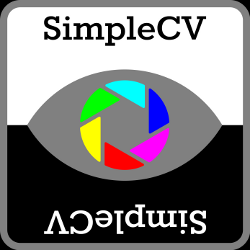
\includegraphics[width=0.5\linewidth]{simplecv.png}
\end{figure}
\end{frame}

% ------------------------------------------------

\begin{frame}
\frametitle{SimpleCV != OpenCV }
\begin{figure}
  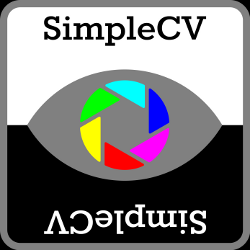
\includegraphics[width=0.2\linewidth]{simplecv.png}
\end{figure}
\begin{itemize}
  \item OpenCV is really busy, we help by wrapping python.
  \item We add lots of other fun stuff (OCR, Barcodes, etc.)
  \item We are not competing, we are complementing. 
  \item Purposes are different. Python is great for prototyping. C++ great for embedded.
\end{itemize}
\end{frame}

% ------------------------------------------------

\begin{frame}
  \frametitle{Core Dependencies}
  \begin{itemize}
  \item \href{http://www.opencv.org}{OpenCV} Python Bindings
  \item \href{http://docs.scipy.org/doc/}{Numpy}
  \item \href{http://docs.scipy.org/doc/}{SciPy}
  \item SciKits Learn and \href{http://orange.biolab.si/}{Orange}
  \item \href{http://www.pygame.org}{PyGame} (this is going away)
  \item \href{http://www.pythonware.com/products/pil/}{Python Imaging Library (PIL)}
  \item \href{http://ipython.org/}{ipython}
  \item PIL (Python Imaging Library)
  \end{itemize}
\end{frame}

% ------------------------------------------------

\begin{frame}
  \frametitle{Optional Dependencies}
  \begin{itemize}
  \item Barcodes- Zebra Crossing \href{https://code.google.com/p/zxing/}{ZXIng}
  \item Optical Character Recognition (OCR) - \href{https://code.google.com/p/tesseract-ocr/}{Tesseract}
  \item Beautiful Soup 
  \item Kinect Support - freenect 
  \item Unit Tests - nose
  \item Web Stuff - flask / CherryPy
  \item Arduino - pyfirmata
  \item Many Many Many more. 
  \end{itemize}
\end{frame}

% ------------------------------------------------

\begin{frame}
  \frametitle{This is why we put everything in a superpack / virtual
    box / bootable drive}
  \begin{itemize}
  \item Just get to the core library functions.
  \item We encourage you to install the full library when you get
    home.
  \item Help is available if you need it. 
  \end{itemize}
\end{frame}

% ------------------------------------------------
\begin{frame}
\frametitle{Getting Help after the tutorial.}
\begin{figure}
  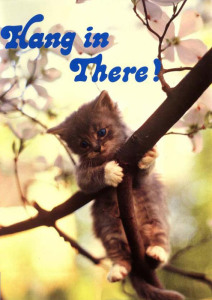
\includegraphics[width=0.2\linewidth]{hang-in-there-cat.jpg}
\end{figure}
\begin{itemize}
  \item Primary Source: \url{http://help.simplecv.org/questions/}
  \item Documentation \url{http://www.simplecv.org/docs/}
  \item Tweet at us: $@$Simple\textunderscore CV
  \item Another Good Resource: \url{http://www.reddit.com/r/ComputerVision}
\end{itemize}
\end{frame}

% ------------------------------------------------
\begin{frame}
\frametitle{On the Printed Page}

 \begin{figure}
%   \begin{subfigure}
     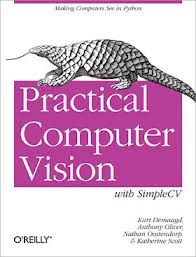
\includegraphics[width=0.4\linewidth]{SimpleCVBook.jpg}
%   \end{subfigure}
%   \begin{sub-figure}
     \quad
     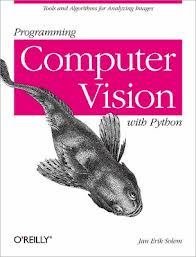
\includegraphics[width=0.4\linewidth]{JanEricBook.jpg}
     \caption{Two books about using Python for Computer Vision}
%   \end{subfigure}
 \end{figure}

\end{frame}

% ------------------------------------------------
\begin{frame}
\frametitle{So why are we doing this?}

\begin{itemize}
  \item We are really nice people who believe in Python and Open
    Source.
  \item We are trying to disrupt industrial quality control systems.
\end{itemize}
\begin{figure}
  
\includegraphics[width=0.6\linewidth]{SightMachineLogo.png}
\end{figure}

\end{frame}

% ------------------------------------------------
\begin{frame}
\frametitle{Early Prototypes}

\begin{figure}
  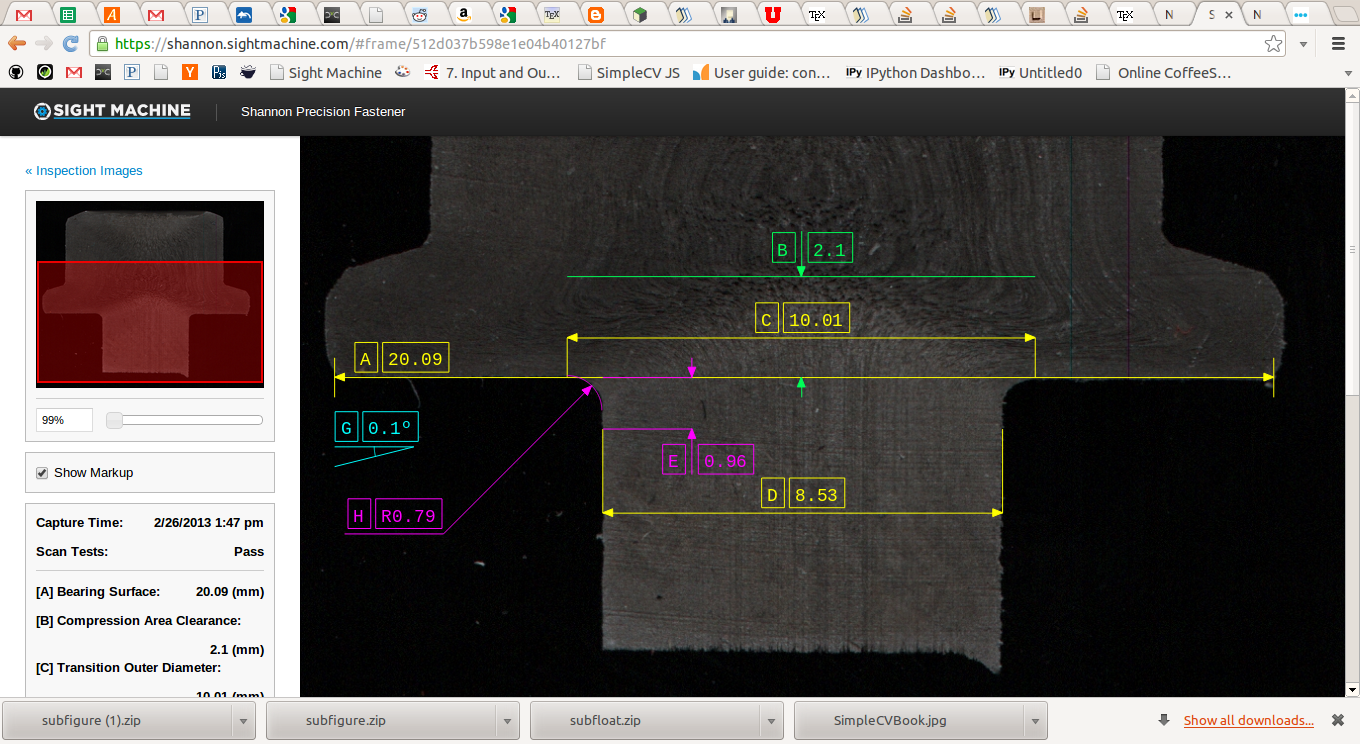
\includegraphics[width=0.8\linewidth]{shannon.png}
  \caption{Early Customer - Industrial Fastener Morphology
      and Metallurgy }
\end{figure}

\end{frame}
% ------------------------------------------------
\begin{frame}
\frametitle{Early Prototypes}

\begin{figure}
  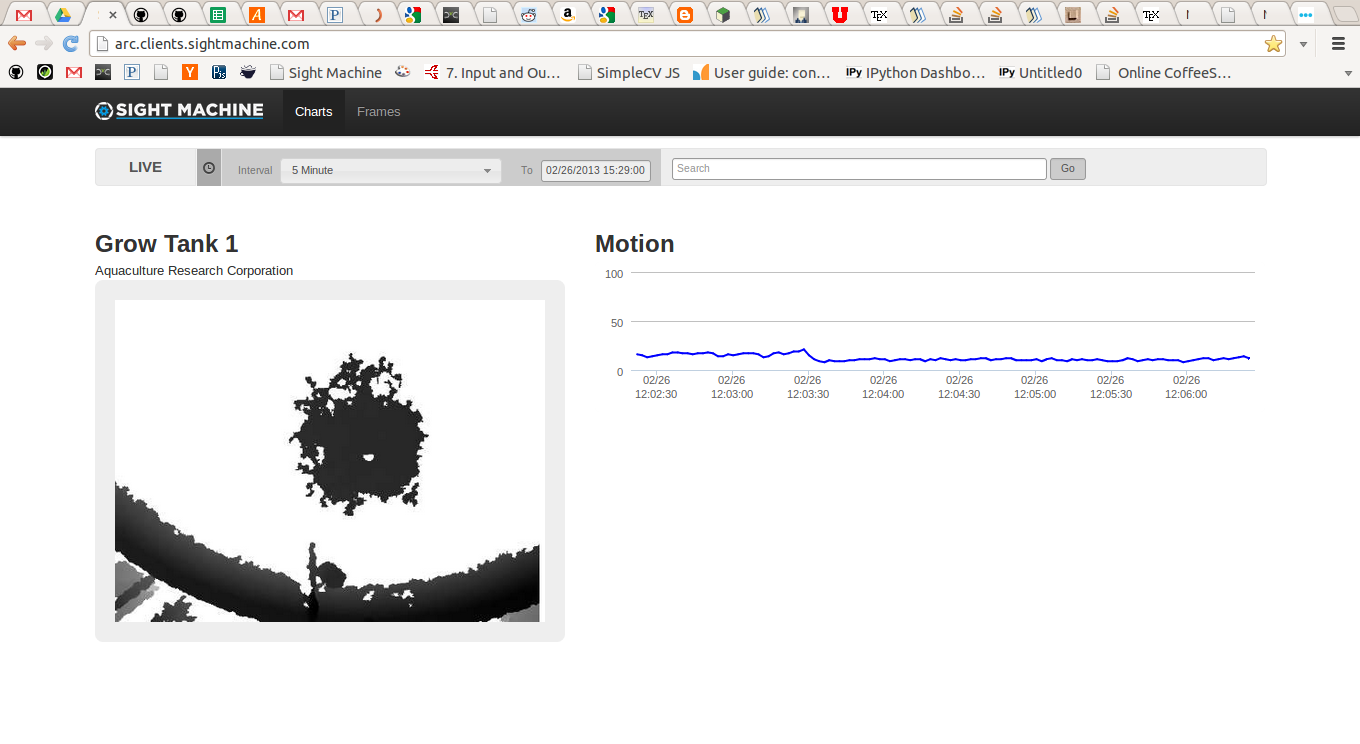
\includegraphics[width=0.9\linewidth]{arc.png}
  \caption{Early Customer - Aquaponics Research Facility}
\end{figure}

\end{frame}

\section{SimpleCV Basics}

% ------------------------------------------------
\begin{frame}
\frametitle{How do I SimpleCV?}

\begin{figure}
  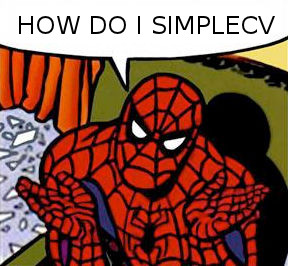
\includegraphics[width=0.4\linewidth]{howdoi.jpg}
\end{figure}

\end{frame}

 
% ------------------------------------------------
\begin{frame}
\frametitle{Where do I write my code?}

\large{So how do I SimpleCV?}
\begin{itemize}
\item In a python file, just like any other library.
\item In a command line REPL like iPython.
\item In the browser using iPython Notebooks (we'll use this today).
\end{itemize}
We really like iPython. It is kinda like using Matlab without the \$ 5000
per seat license cost. 
\end{frame}

%------------------------------------------------

\begin{frame}
\frametitle{How does fit into a work flow?}
At SightMachine we roughly use these three tools 
for different parts of our workflow.
\begin{table}
\begin{tabular}{l l }
\toprule
\textbf{Tool} & \textbf{Uses} \\
\midrule
iPython REPL & Prototypes, Sanity Checks, Etc \\
iPython Web Notebook & Testing and Development \\
Python Files  & Deployment Code \\
\bottomrule
\end{tabular}
\caption{SimpleCV Workflow}
\end{table}
\end{frame}


% ------------------------------------------------

\begin{frame}[fragile] % Need to use the fragile option when verbatim is used in the slide
\frametitle{SimpleCV Hello World as a Script}
\begin{example}[HelloWorld.py]
 \inputminted[linenos=true, tabsize=4,
 fontsize=\small]{python}{HelloWorld.py}
\end{example}
\end{frame}
% ------------------------------------------------
\begin{frame}
\frametitle{How do I run Hello World?}
\begin{itemize}
\item Run the py file with $python$ $HelloWorld.py$ in the command.
\item Close it by pressing $esc$ or $ctrl-c$
\end{itemize}
\begin{figure}
  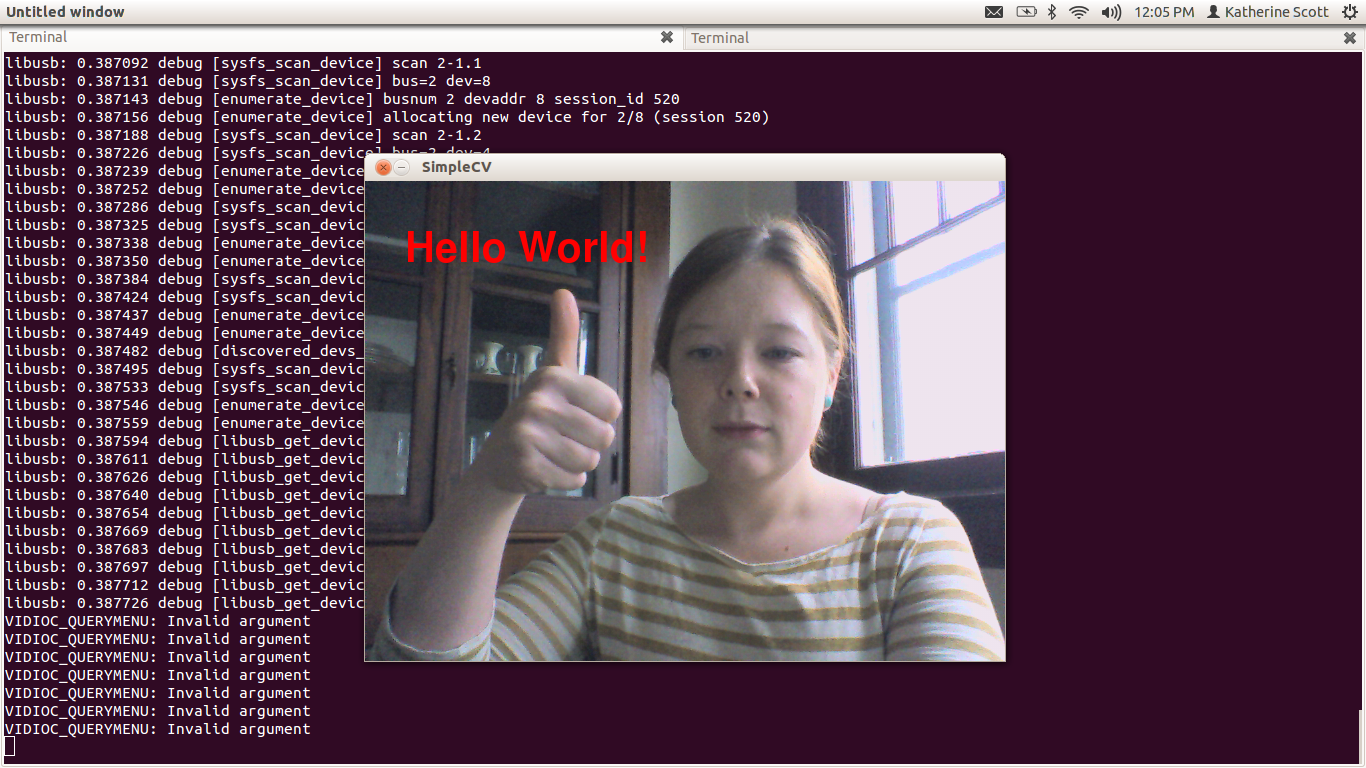
\includegraphics[width=0.8\linewidth]{HelloWorld1.png}
\end{figure}
\end{frame}

% ------------------------------------------------
\begin{frame}
\frametitle{The SimpleCV Shell - Custom iPython REPL}
Sometimes you just want to test an idea without writing a full
script. For this reason we created the SimpleCV shell, which is a
custom ipython instance. The SimpleCV shell will allow you to:
\begin{itemize}
\item Test your ideas in a REPL similar to Matlab.
\item Access the SimpleCV documentation. 
\item Import modules that you are working with to test.
\item Run through an interactive tutorial. 
\end{itemize}
\end{frame}

%------------------------------------------------
\subsection{SimpleCV Shell}
\begin{frame}[fragile] % Need to use the fragile option when verbatim is used in the slide
\frametitle{Starting the SimpleCV Shell}
In OSX and Linux just type $simplecv$ at the command line. On Windows
you just click on the SimpleCV icon. 
\begin{example}[Shell Basics]
\begin{minted}[fontsize=\tiny]{python}
+-----------------------------------------------------------+
 SimpleCV 1.3.0 [interactive shell] - http://simplecv.org
+-----------------------------------------------------------+
Commands: 
	"exit()" or press "Ctrl+ D" to exit the shell
	"clear" to clear the shell screen
	"tutorial" to begin the SimpleCV interactive tutorial
	"example" gives a list of examples you can run
	"forums" will launch a web browser for the help forums
	"walkthrough" will launch a web browser with a walkthrough
Usage:
	dot complete works to show library
	for example: Image().save("/tmp/test.jpg") will dot complete
	just by touching TAB after typing Image().
Documentation:
	help(Image), ?Image, Image?, or Image()? all do the same
	"docs" will launch webbrowser showing documentation
\end{minted}
\end{example}
\end{frame}
%------------------------------------------------
\begin{frame}
\frametitle{SimpleCV Shell Like a Boss}
\begin{figure}
  
\includegraphics[width=0.3\linewidth]{protip.jpg}
\end{figure}
\begin{itemize}
\item Putting a ? in front of a class or method will give you
  documentation. The ``/'' key will let you search.
\item iPython has tab completion for methods.
\item Up arrow will give you previous commands. 
\item \%paste will let you paste formatted code. 
\item Other cool stuff can be found by googling iPython magic commands.
\end{itemize}
\end{frame}

%------------------------------------------------
\begin{frame}[fragile] 
\frametitle{Let's repeat Hello World  in SimpleCV  Shell}
\begin{example}[In the SimpleCV shell]
\begin{minted}[fontsize=\small]{python}
SimpleCV:1> cam = Camera()
SimpleCV:2> disp = Display((640,480))
SimpleCV:3> while disp.isNotDone():
       ...:     img = cam.getImage().edges()
       ...:     img.drawText("Hello World!",40,40,fontsize=60)
       ...:     img.save(disp)
       ...:     
SimpleCV:4> exit
\end{minted}
\end{example}
\begin{itemize}
\item Just push return after each line.
\item iPython will do tabbing in the while loop.
\item $esc$ to quit or $ctrl-c$.
\item type ``exit'' to quit.
\end{itemize}
\end{frame}
% ------------------------------------------------
\begin{frame}
\frametitle{Yes, it really is that simple.}
\begin{figure}
  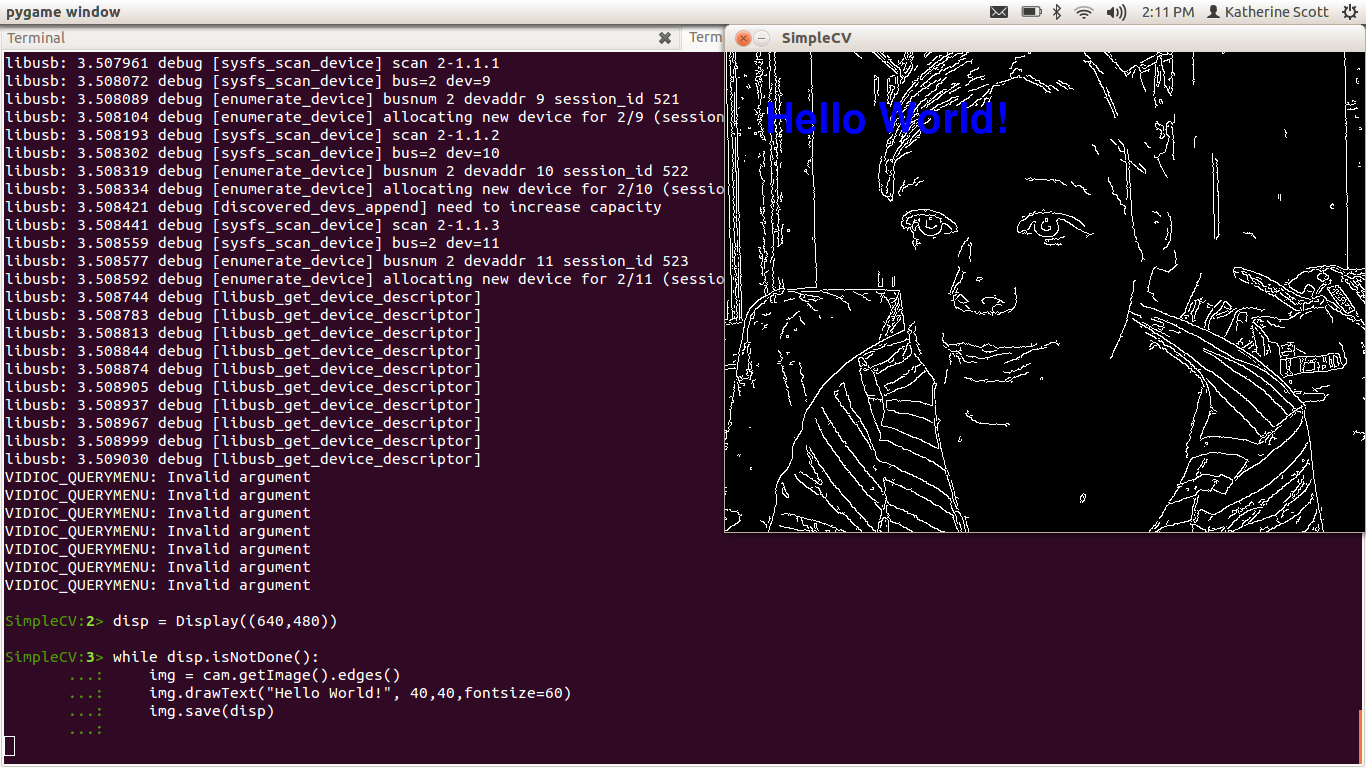
\includegraphics[width=0.9\linewidth]{HelloWorld2.png}
\end{figure}
\end{frame}
% ------------------------------------------------
\subsection{iPython Web Notebook}
% ------------------------------------------------
% ------------------------------------------------
\begin{frame}
\frametitle{Why use iPython Web Notebooks}
\begin{figure}
  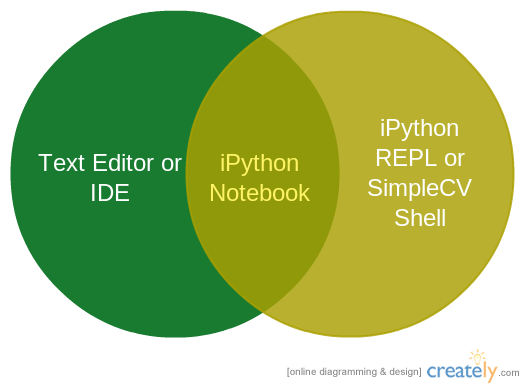
\includegraphics[width=0.4\linewidth]{venn.png}
\end{figure}
\begin{itemize}
\item Web notebooks give you the best features of an IDE and a REPL.
\item You can edit chunks of code, and then execute them in series.
\item iPython is still v. 0.1.4 but it is getting good fast.
\end{itemize}
\end{frame}
% ------------------------------------------------
\begin{frame}
\frametitle{How do I use the notebook?}
\begin{figure}
  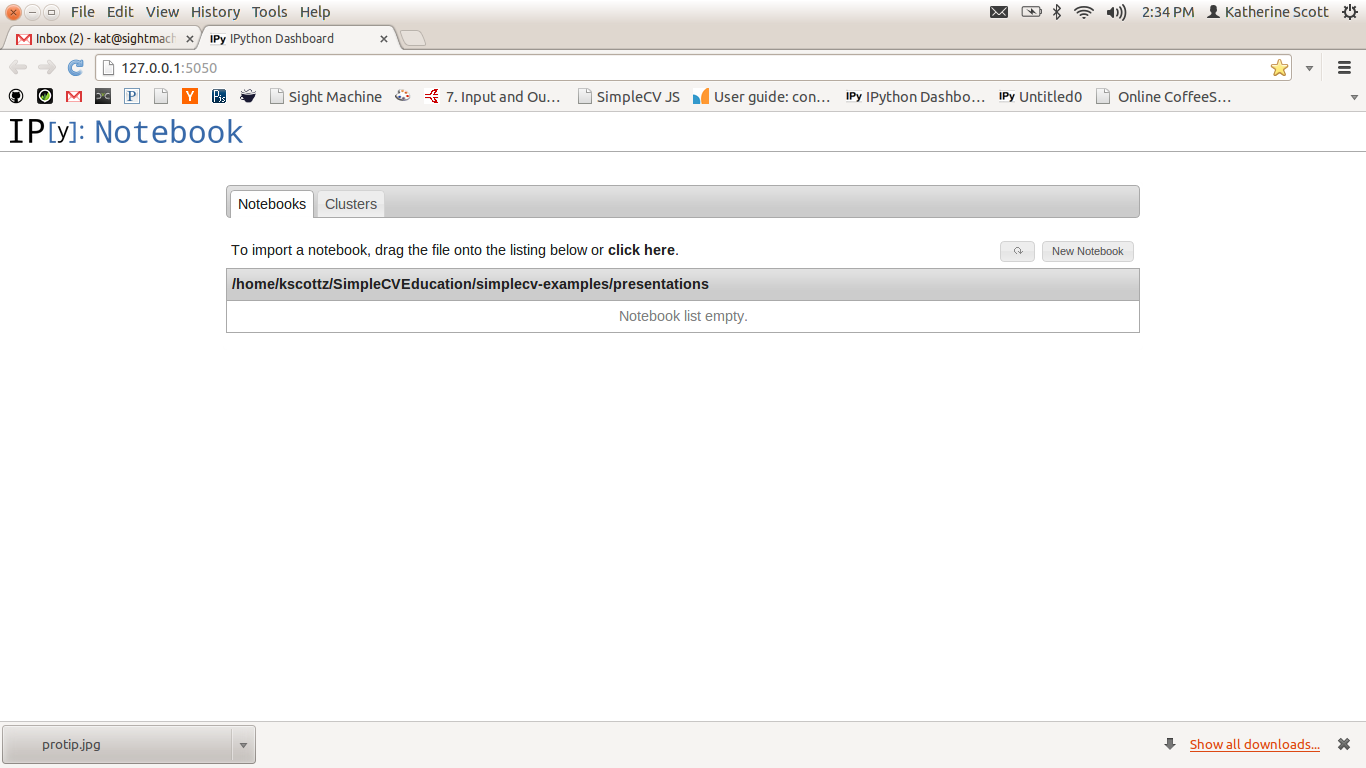
\includegraphics[width=0.5\linewidth]{startingipython.png}
\end{figure}
\begin{itemize}
\item From the shell just type $simplecv$ $notebook$ $--pylab$
  $inline$.
\item The --pylab inline is optional but it pulls in matplotlib which
  is handy.
\item You will get to a dashboard to create a new notebook.
\item By default notebooks are in the path where you start ipython.
\end{itemize}
\end{frame}
% ------------------------------------------------
\begin{frame}
\frametitle{How do I use the notebook?}
\begin{figure}
  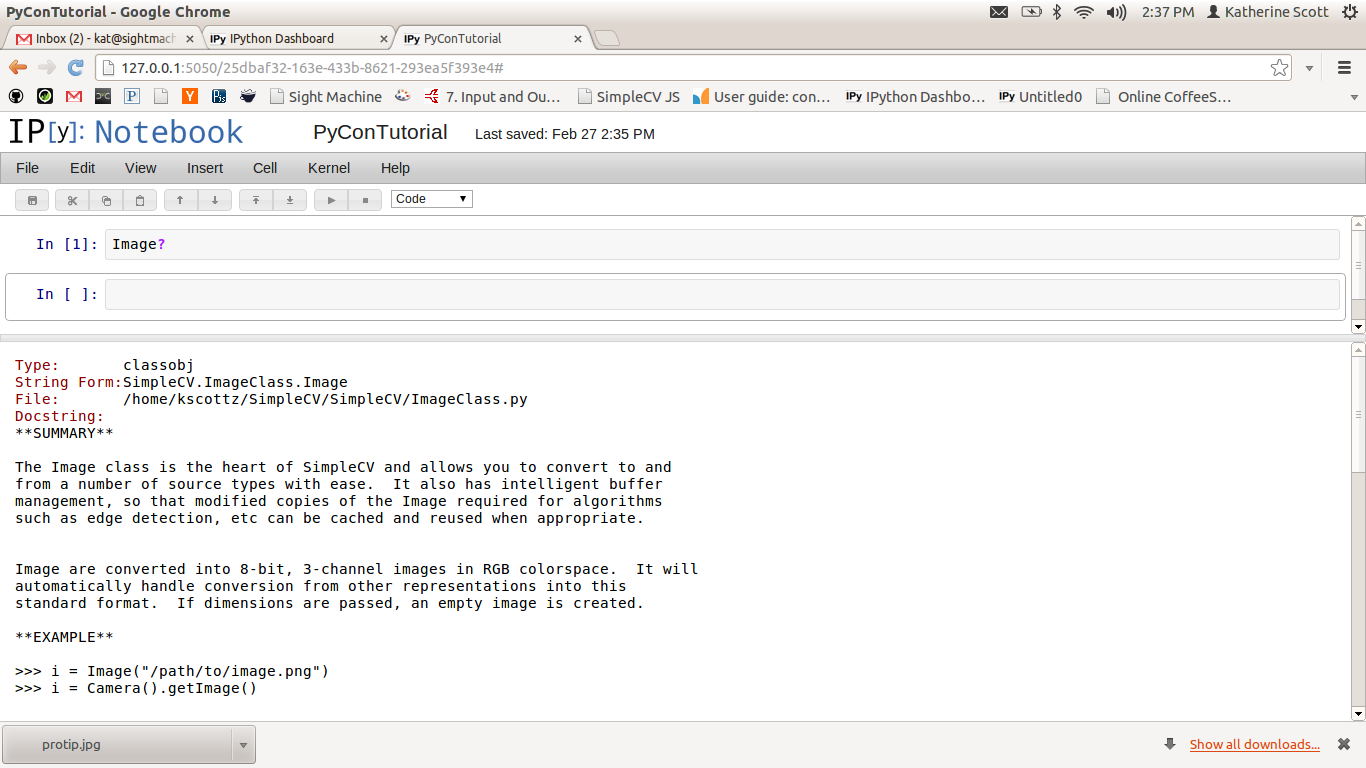
\includegraphics[width=0.7\linewidth]{ipythonHelp.png}
\end{figure}
\begin{itemize}
\item Everything we mentioned about the SimpleCV shell still holds.
\item Magic commands, inline documentation, etc. still work.
\item $enter$ starts a new line.
\item $ctrl-enter$ executes a line.
\end{itemize}
\end{frame}
% ------------------------------------------------
\begin{frame}
\frametitle{Caveats about  iPython Web Notebooks}
\begin{figure}
  
\includegraphics[width=0.2\linewidth]{warning.jpg}
\end{figure}
\begin{itemize}
\item iPython Web Notebooks are still version 0.1.4 
\item \textbf{There is no auto-save. Get in the $ctrl-s$ save habit.}
\item If you edit a module you import you must restart the core. 
\item Minimal editing support. No find/replace.
\item The core can sometimes crash on large images.
\item The notebooks hold on to data by default. This can fill up your
  version control system fast. Try the download as python command from
  the gui. 
\end{itemize}
\end{frame}
% ------------------------------------------------
% ------------------------------------------------
% ------------------------------------------------
 \section{Image Basics}
% % ------------------------------------------------
% % ------------------------------------------------
% % ------------------------------------------------
\begin{frame}
\frametitle{Image Loading Basics II}
\begin{itemize}
\item You can get the image file name using $img.filename$
\item Images can also come from appropriately shaped numpy arrays.
\item PIL and OpenCV images can also be passed into the image.
\item Can also take a URL to an image. 
\item The \textbf{img.getEXIFData()} command can show jpg EXIF data.
\end{itemize}
\end{frame}

% % ------------------------------------------------
\begin{frame}
\frametitle{Saving an Image}
\begin{itemize}
\item The \textbf{img.save()} command is used to save images.
\item You can save as just about any format, PNG, JPG, WebP, etc.
\item Calling save with no parameters saves it to temp directory.
\item Using the params flag you can set compression, e.g. set
  compression quality. 
\end{itemize}
\end{frame}

% % %------------------------------------------------
\begin{frame}
\frametitle{Using a USB Camera}
\begin{itemize}
\item Most usb cameras use the \textbf{Camera} class. 
\item The camera class takes a camera index, \emph{usually} this is the
   order cameras are plugged into the computer.
\item The camera also has properties that you can get and set, or use a propmap dictionary to set. 
 \item \textbf{Support for camera properties is vendor specific and spotty at
   best.} 
 \item Cameras also have a \textbf{threaded} parameter. Set this to false
 to run multiple cameras. 
\end{itemize}
\end{frame}
% ------------------------------------------------
\begin{frame}
\frametitle{Using a USB Camera II}
\begin{itemize}
\item \textbf{Camera.getImage()} will return the current image. 
\item \textbf{Camera.getAllProperties()} will return the cameras properties.
\item \textbf{Camera.getProperty() and Camera.setProperty()} may let
  you set properties. \emph{This is highly vendor dependent and usually poorly documented.}
\end{itemize}
\end{frame}
%------------------------------------------------
\begin{frame}
\frametitle{Briefly: Other Cameras}
\begin{itemize}
\item Kinect - Depth Camera
\begin{itemize}
\item Uses freenect drivers, not the OpneNI drivers.
\item \textbf{Kinect.getImage and Kinect.getDepth }
\item Note that these aren't well calibrated together.
\end{itemize}
\item JpegStreamReader - IP Cameras
\begin{itemize}
\item Give it a url to camera's web feed, and scrape images.
\item Getting the URL straight can be tricky. 
\end{itemize}
\item Virtual Camera
\begin{itemize}
\item A virtual camera that pulls from a directory full of images, or video.
\item Interface to video files for processing.
\end{itemize}
\end{itemize}
\end{frame}
% ------------------------------------------------
\begin{frame}
\frametitle{Briefly: Other Cameras}
\begin{itemize}
\item Document Scanners
\begin{itemize}
\item SANE compatible devices.
\item Allow you to set resolution and ROI. 
\end{itemize}
\item Digital Camera
\begin{itemize}
\item Uses Piggy Photo Library
\item Works with most DSLRs and point and shoots.
\end{itemize}
\item AVT Camera
\begin{itemize}
\item Professional digital imaging cameras with interchangeable optics.
\item Fine grain control of camera parameters. 
\end{itemize}
\end{itemize}
\end{frame}
% ------------------------------------------------
\begin{frame}
\frametitle{Image Sets}
ImageSets are lists of images. They are great for aggregating datasets.
\begin{itemize}
\item By default load all image files in a directory.
\item Can iterate over the list using list comps or for loops.
\item Using the BeautifulSoup library can download sets from google.
\item Can save image sets to directories, or animated gifs!
\item The show command works just like on image class.
\item Can apply averages to images.
\item More coming soon.
\end{itemize}
\end{frame}

% ------------------------------------------------
\begin{frame}[fragile] 
\frametitle{ImageSet Example}
\begin{example}[Image Sets]
\begin{minted}[fontsize=\small]{python}
mySet = ImageSet()
mySet.download('cats') # download cats
mySet.show() # show them to us
avgCat = mySet.average() # get the avg cat
avgCat.show() # show the avg cat
mySet[3].show() # show the third kitty
resized = mySet.standardize(128,64)
resized.save('cat.gif')
mySet.save('cat.gif') # save the cats as a gif
for cat in mySet: # iterate over the set of cats
    cat.binarize().show()
\end{minted}
\end{example}
\end{frame}
% ------------------------------------------------
\section{Really Basic Operations}
\begin{frame}
\frametitle{Getting at a pixel}
\begin{figure}
  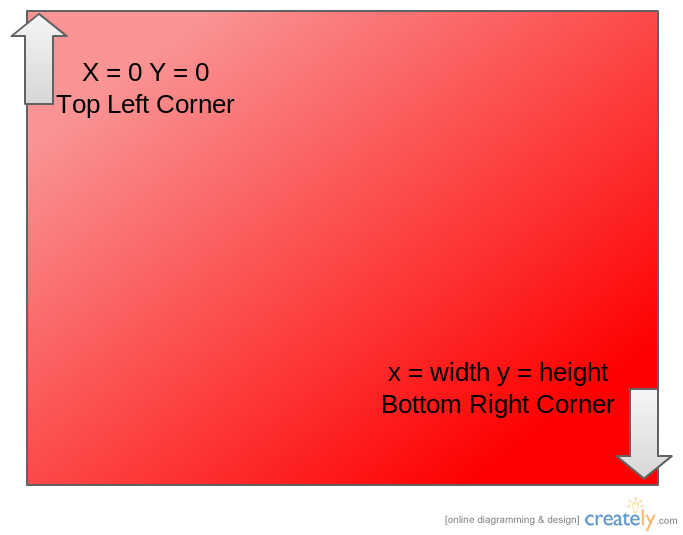
\includegraphics[width=0.5\linewidth]{pixellocations.png}
\end{figure}
\begin{itemize}
\item SimpleCV treats images as two dimensional arrays of color
value tuples. 
\item Each tuple holds three values (Red,Green,Blue).
\item Pixels start in the top left corner at zero. 
\end{itemize}
\end{frame}

% ------------------------------------------------
\begin{frame}[fragile] 
\frametitle{Pixel Manipulation Example}
\begin{example}[Getting at those pixels]
\begin{minted}[fontsize=\small]{python}
img = Image('helloworld.jpg')
c = img[0,0] # get a pixel
print c
print img.getPixel(0,0) # get another way
test = img[200:300,200:300]
test.show() # the result is an image
test = img[50:,:]
test.show() # again using slice
test = img[0:5,0:5]
print test.getNumpy() # get the raw values
img[0:105,0:105] = Color.RED 
img.show() # Another way
test = img.getNumpy() #RIGHT!
test[0:105,0:105] = Color.RED
img2 = Image(test)
img2.show()
\end{minted}
\end{example}
\end{frame}
% ------------------------------------------------
\begin{frame}
\frametitle{Getting at a pixel}
\begin{itemize}
\item Images are read only. To write a pixel directly you need create a new
  image. Usually this happens in numpy
\item Images support the list slice notation but return images.
\item To get at the raw pixel values use \textbf{getNumpy()} and \textbf{getGrayNumpy()} 
\item Numpy values can be accessed using slices the first parameter is
  x, the second is y,  and the third is the channel in RGB order. For
  example $npimg[x][y][0]$. 
\item The \textbf{Image.width} and \textbf{Image.height} member
  variables can help you find your way. 
\end{itemize}
\end{frame}
% ------------------------------------------------
\begin{frame}[fragile] 
\frametitle{Another Pixel Manipulation Example}
\begin{example}[Fancy Manipulations]
\begin{minted}[fontsize=\tiny]{python}
img = Image('helloworld.jpg')
gray = img.getGrayNumpy() # get the gray scale np image
colored = img.getNumpy()  # and the colored one
print (img.width,img.height) #tell us the image size
colored[0:20,:] = Color.BLUE # set the left side to blue
colored[:,0:20] = Color.GREEN # set the top row to green
colored[40:80,40:80]      \quad
     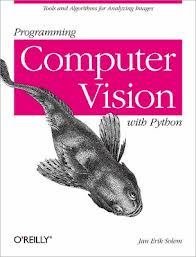
\includegraphics[width=0.4\linewidth]{JanEricBook.jpg}
= Color.YELLOW # make a yellow square
x,y = np.where(gray>230) # find bright pixels > 230
for xf,yf in zip(x,y): # for each of those
    colored[xf][yf] = Color.RED #make them red
img2 = Image(colored) # create an image
img2.show() # and show it
# now set the whole blue channel to 255
colored[:,:,2] = 255 
# and show us that
img3 = Image(colored)
img3.show()
\end{minted}
\end{example}
\end{frame}
% ------------------------------------------------
\begin{frame}
\frametitle{Getting at a pixel}
 \begin{figure}
     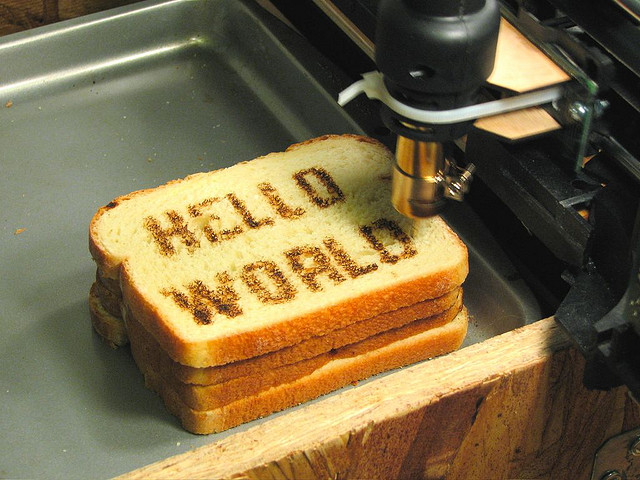
\includegraphics[width=0.3\linewidth]{helloworld.jpg}
     \quad
     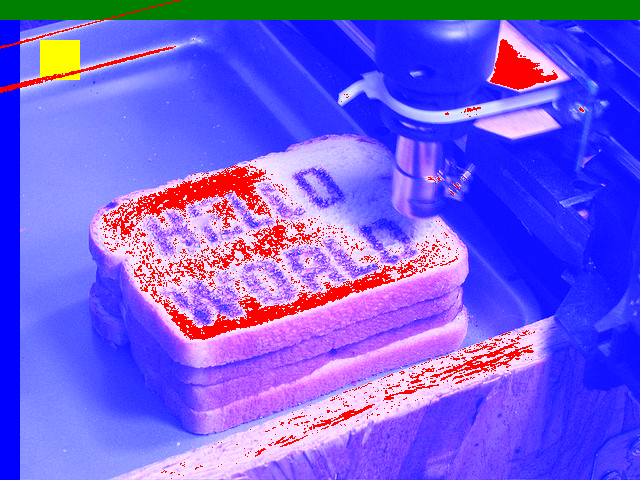
\includegraphics[width=0.3\linewidth]{ColorToast.png}
     \quad
     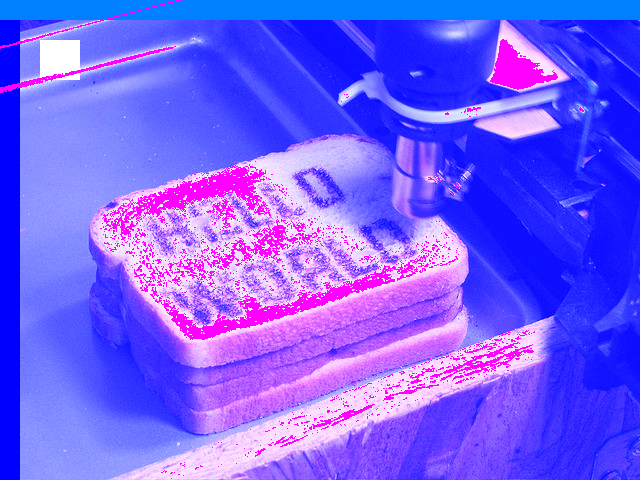
\includegraphics[width=0.3\linewidth]{ColorToast2.png}
     \caption{Not bad for less than 20 lines of code.}
 \end{figure}

\end{frame}
% ------------------------------------------------
\section{Basic Manipulations}
% ------------------------------------------------
\begin{frame}
\frametitle{Cropping, Scaling, Rotating, etc}
It is helpful to think of some image processing like using an image
editor, like GIMP, paint, or that other one Adobe makes. Here are a
few basic image operations you can do in SimpleCV. 
\begin{itemize}
\item \textbf{Image.crop}. Does what it says on the tin. We refer to
  crop areas by there top left corner x and y plus the width height.
\item \textbf{Image.scale} scales the image proportionally while
  \textbf{Image.resize} resizes the image to the desired size. 
  \begin{itemize}
    \item \textbf{Image.resize} is smart, if you tell it a width or
      height it will infer the other parameter from the aspect ratio.
    \item \textbf{Image.scale} uses a proportionality. So passing it
      value of two will double the image size. Make sure to check out
      the interpolation method.
  \end{itemize}
\end{itemize}
\end{frame}
% ------------------------------------------------
\begin{frame}
\frametitle{Rotating}
\begin{itemize}
  \item \textbf{Image.rotate} takes and angle in degrees.
  \item Rotate has a parameter called fixed. If fixed
        is set to false, SimpleCV will create a new image that matches
        the rotated image size. Otherwise we stick the rotated image
        in data in a similarly sized canvas. 
  \item It is possible to pick the x,y position of the rotation. The
    default is the center of the image.
  \item You can also scale an image while rotating.
  \item In a pinch you can use \textbf{Image.flipHorizontal} and
    \textbf{Image.flipVertical}.
   \item Be aware \textbf{FLIPPING != ROTATION}
\end{itemize}
\end{frame}
% ------------------------------------------------
\begin{frame}
\frametitle{Blit}
The \textbf{Image.blit} function gets its name from the old computer graphics term ``bit block image
transfer''. Really it means just copy and paste another image onto
another image and return the result.
\begin{itemize}
\item Blit takes in another image and a position where you want to put
  it.
\item That position can be negative with respect to the destination
  image. For example (-10,-10) would put the source image over the top
  left of the destination image.
\item You can toss blit a binary mask, an alpha value (that is
  transparency) or a an alpha mask (a grayscale image that has an
  alpha mask per pixel).
\end{itemize}
\end{frame}
% ------------------------------------------------
\begin{frame}[fragile] 
\frametitle{Let's play!}
\begin{example}[Basic Manipulations]
\begin{minted}[fontsize=\tiny]{python}
img = Image('tricky.jpg')
face = img.crop(150,190,309-150,333-190)
img.show() # show the source
face.show() # show the cropped image
face.rotate(45).show() # basic rotation
face.rotate(45,fixed=False).show()
face.scale(0.5).show()
face.scale(width=int(face.width/2.0)) # basic scaling
face.flipHorizontal().show() # flipping
test1 = img.blit(face.flipHorizontal(),pos=(150,190))
test1.show() # now let's have fun with blitting
test2 = img.blit(face.flipHorizontal(),pos=(150,190),alpha=0.5)
test2.show() 
mask = Image((face.width,face.height))
# Here we are just drawing a white circle on a black background
mask.drawCircle((face.width/2,face.height/2),70,color=Color.WHITE, thickness=-1)
mask = mask.applyLayers()
mask.show()
test3 = img.blit(face.flipHorizontal(),pos=(150,190),mask=mask)
test3.show()
face.binarize().blur().show()
test4 = img.blit(face.flipHorizontal(),pos=(150,190),alphaMask=face.binarize().blur())
test4.show()
\end{minted}
\end{example}
\end{frame}
% ------------------------------------------------
\begin{frame}
\frametitle{The Blit Progression of President Dick Nixon}
 \begin{figure}
     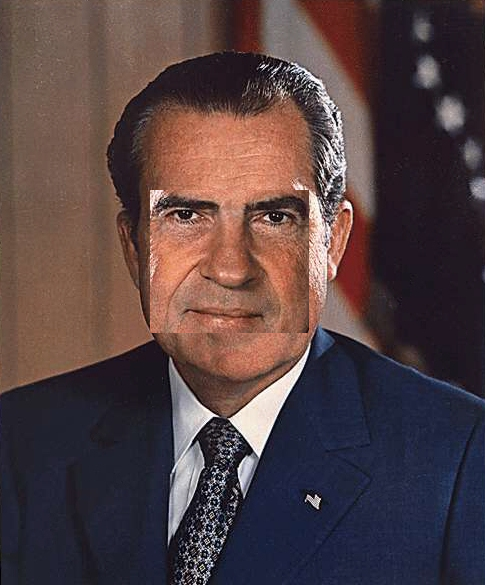
\includegraphics[width=0.2\linewidth]{tricky1.png}
     \quad
     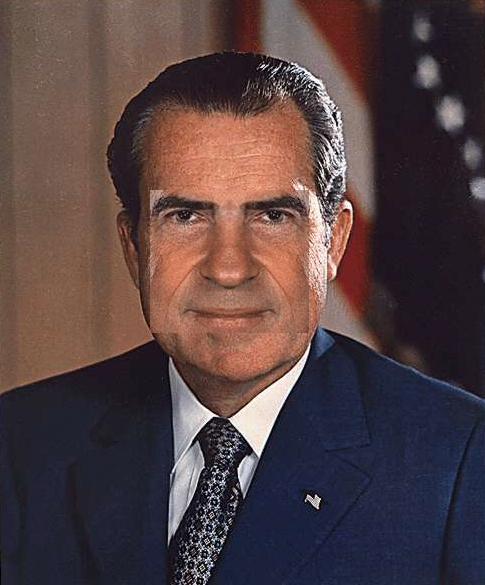
\includegraphics[width=0.2\linewidth]{tricky2.png}
     \quad
     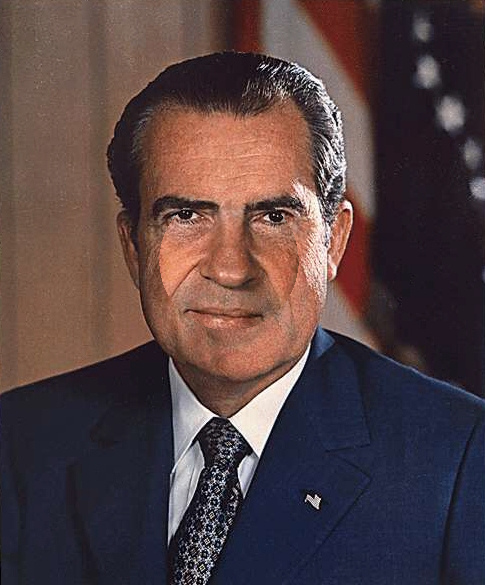
\includegraphics[width=0.2\linewidth]{tricky3.png}
     \quad
     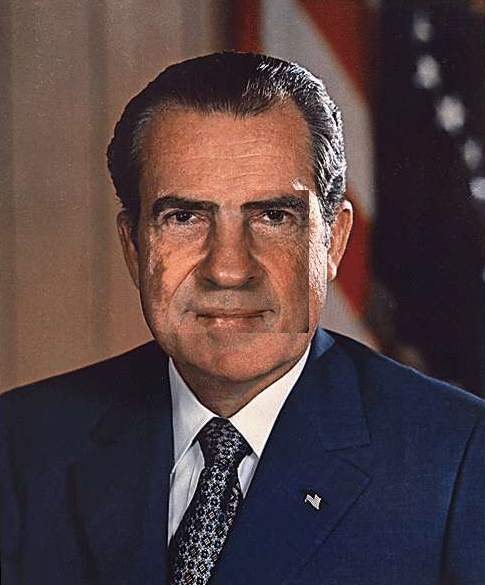
\includegraphics[width=0.2\linewidth]{tricky4.png}
     \quad
     \caption{Various blitting}
 \end{figure}
\large{Can you our subject a smaller face or a slightly slanted face? }
\end{frame}
% ------------------------------------------------
\begin{frame}
\frametitle{A few more basics}
\begin{itemize}
  \item \textbf{Image.blur} - A basic Gaussian blur. 
  \item \textbf{Image.smooth} - A variety of smoothing filters. Some
    good for removing camera noise. 
  \item \textbf{Image.toGray} - Convert a color image to a gray scale
    image.
  \item \textbf{Image.threshold} - Take an image and set all off the
    pixels that have a grayscale value above the threshold to white,
    and everything else to black.
 \item \textbf{Image.invert} - Swap the lightest and darkest values,
   like a photo negative. 
\end{itemize}
\end{frame}
% ------------------------------------------------
\section{Rendering Information}
\begin{frame}
\frametitle{SimpleCV treats on image rendering as a separate layer.}
\begin{itemize}
  \item Each image has a stack of transparent drawing layers. 
  \item Every time you call a draw command we draw on the transparent layer.
  \item This is layer is rendered when you call the
    \textbf{Image.show} command or save it to a display.
  \item \textbf{Image.save} does not save the drawing layer by default.
 \item Use the \textbf{Image.applyLayers} command to return a new
   image with the layer applied.
   \item The \textbf{Image.clearLayers} command removes the layers.
\end{itemize}
\end{frame}
% ------------------------------------------------
\begin{frame}
\frametitle{Accessing the drawing layer.}
\begin{itemize}
  \item \textbf{Image.dl} method returns the drawing layer that has
      more advanced rendering features. 
  \item The drawinglayer is really a list of layers if you need them.
  \item You can set the layer alpha value. 
  \item Allows for more fine grained control.
  \item Use sprite for non-destructive blit function.
  \item Use the \textbf{Color} class for colors or set your own. 
\end{itemize}
\end{frame}

% ------------------------------------------------
\begin{frame}
\frametitle{Basic Drawing Primitives}
\begin{itemize}
  \item \textbf{Image.drawCircle} - Draw a circle based on center and radius.
  \item \textbf{Image.drawRectanle} - Draw a rectangle on top left
    corner and width and height.
  \item \textbf{Image.drawRotatedRectangle} - Draw rectangle from
    rotated points.
  \item \textbf{Image.drawText} - Draw a line of text at a position
  \item \textbf{Image.drawLine} - Draw a line based on two (x,y) points.
  \item \textbf{Image.drawPoints} - Put a circle around points of
    interest. 
\end{itemize}
\end{frame}
% ------------------------------------------------
\begin{frame}[fragile] 
\frametitle{Go crazy with drawing.}
\begin{example}[Basic Manipulations]
\begin{minted}[fontsize=\tiny]{python}
img = Image('tricky.jpg')
poly = [(0,0),(30,50),(123,213),(234,234),(333,434)]
img.dl().polygon(poly,color=Color.GREEN,filled=True)
for i in xrange(30,90,9):
    poly2 = [(p[0]+i,p[1]+i) for p in poly]
    img.dl().polygon(poly2,color=Color.getRandom(),filled=True,alpha=128)
img.drawRectangle(130,190,200,50,color=Color.BLACK,width=-1,alpha=128)
img.drawCircle((170,220),20,color=Color.WHITE)
img.drawCircle((230,220),20,color=Color.WHITE)
img.drawLine((0,0),(100,100),color=Color.PUCE,thickness=3)
img.drawLine((300,200),(300,200),color=Color.PUCE,thickness=3)
img.drawLine((45,300),(300,45),color=Color.PUCE,thickness=3)
img.drawText('HELLO WORLD!',30,30,fontsize=60)
img.show()
img.applyLayers().save('crazynixon.png')
img.clearLayers()
img.show()
\end{minted}
\end{example}
\end{frame}
% ------------------------------------------------
\begin{frame}
\frametitle{Crazy Drawing Stuff.}
 \begin{figure}
     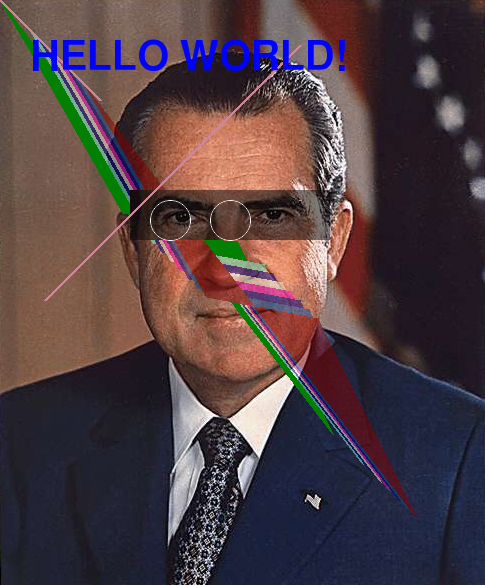
\includegraphics[width=0.5\linewidth]{crazynixon.png}
     \caption{Various drawing things.}
 \end{figure}
\end{frame}
% ------------------------------------------------


\section{Let's talk about black, white, and color}
% ------------------------------------------------
\begin{frame}
\frametitle{Let's Talk about color, color spaces, and much more.}
 \begin{figure}
     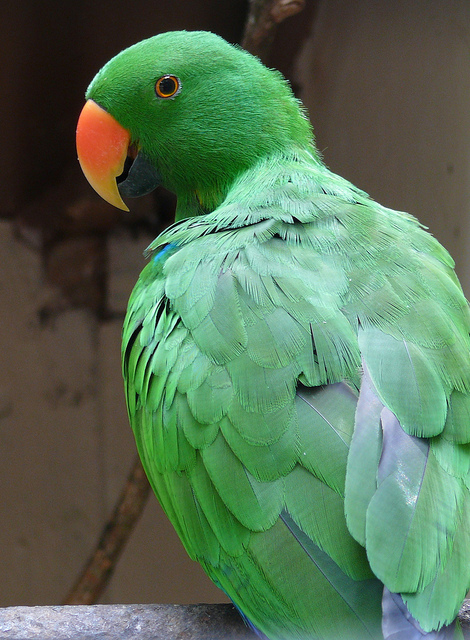
\includegraphics[width=0.2\linewidth]{parrot.jpg}
     \quad
     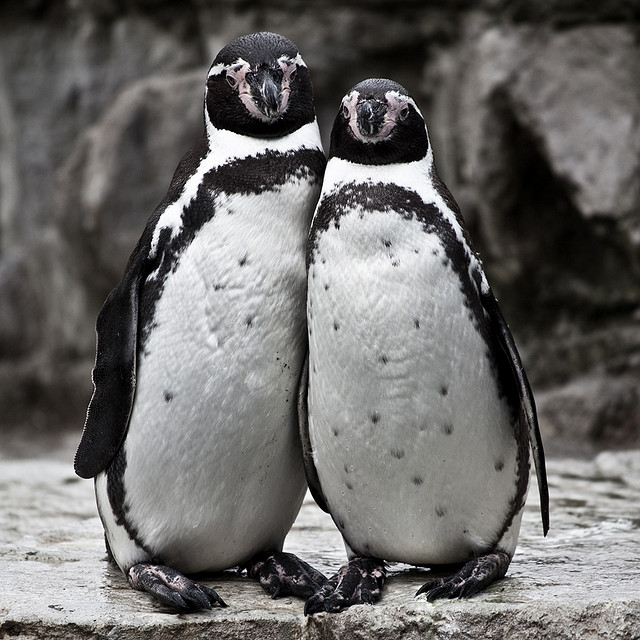
\includegraphics[width=0.3\linewidth]{penguins.jpg}
 \end{figure}
Computer vision is all about moving from a vast amount of
information to small result as quickly as possible. Working in
grayscale, or black and white images can speed things up
dramatically. 
\end{frame}

% ------------------------------------------------
\begin{frame}
\frametitle{Color is surprisingly hard to represent}
 \begin{figure}
     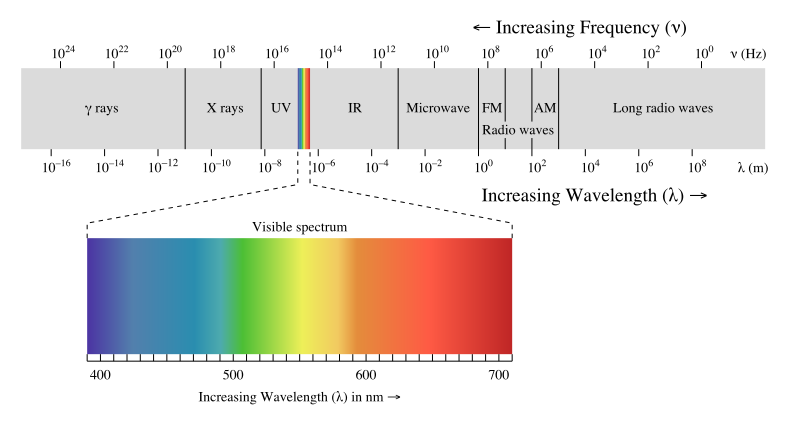
\includegraphics[width=0.3\linewidth]{visiblelight.png}
     \quad
     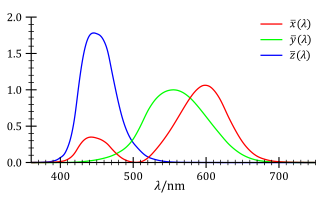
\includegraphics[width=0.3\linewidth]{theeye.png}
     \quad
     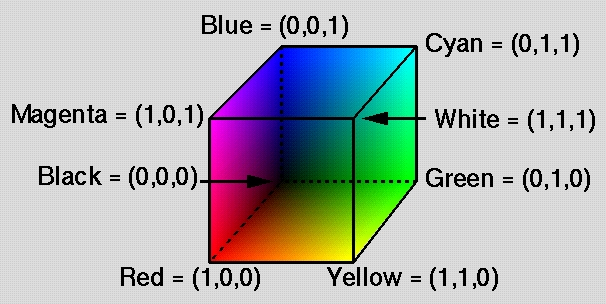
\includegraphics[width=0.3\linewidth]{RGB_cube_color.jpg}
 \end{figure}
We start with visible light, which bounces around, does funky stuff, and then enters our
eye or camera. Our eyes and cameras have a response function that does
an imperfect job of sampling the parts of the spectrum. We then take
those samples and try to map them onto finite color space like RGB. 
\end{frame}

% ------------------------------------------------
\begin{frame}
\frametitle{An illustration of why color is hard.}
 \begin{figure}
     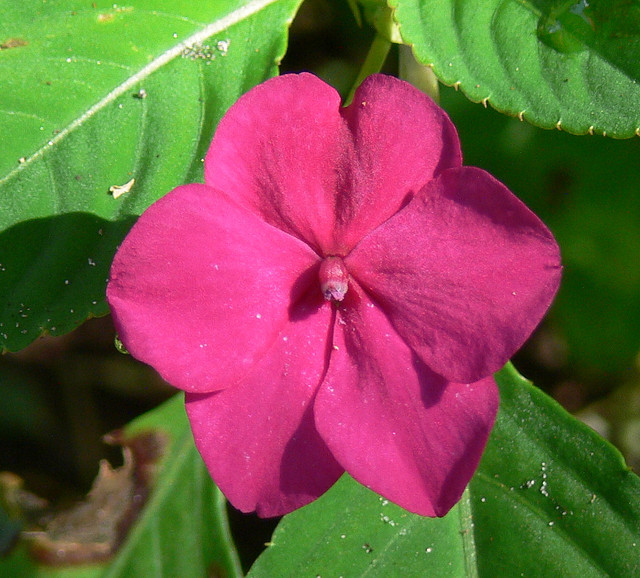
\includegraphics[width=0.3\linewidth]{flower.jpg}%
     \quad
     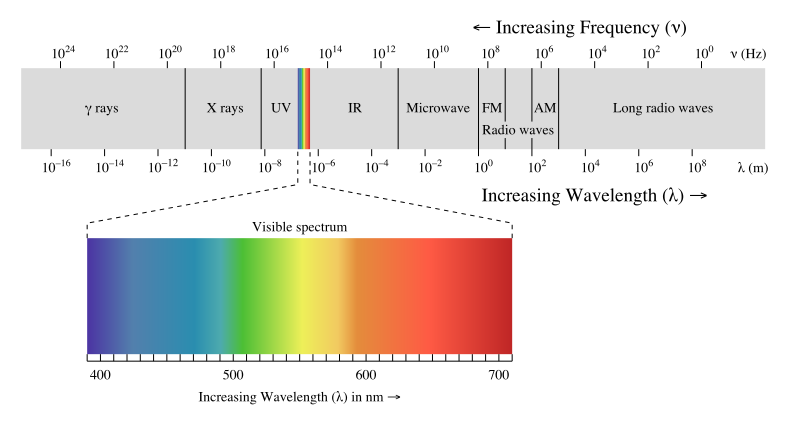
\includegraphics[width=0.5\linewidth]{visiblelight.png}%
 \end{figure}
Point to where this magenta flower lives on the visible light spectrum.
\end{frame}
% ------------------------------------------------
\begin{frame}
\frametitle{MIND BLOWN!}
 \begin{figure}
     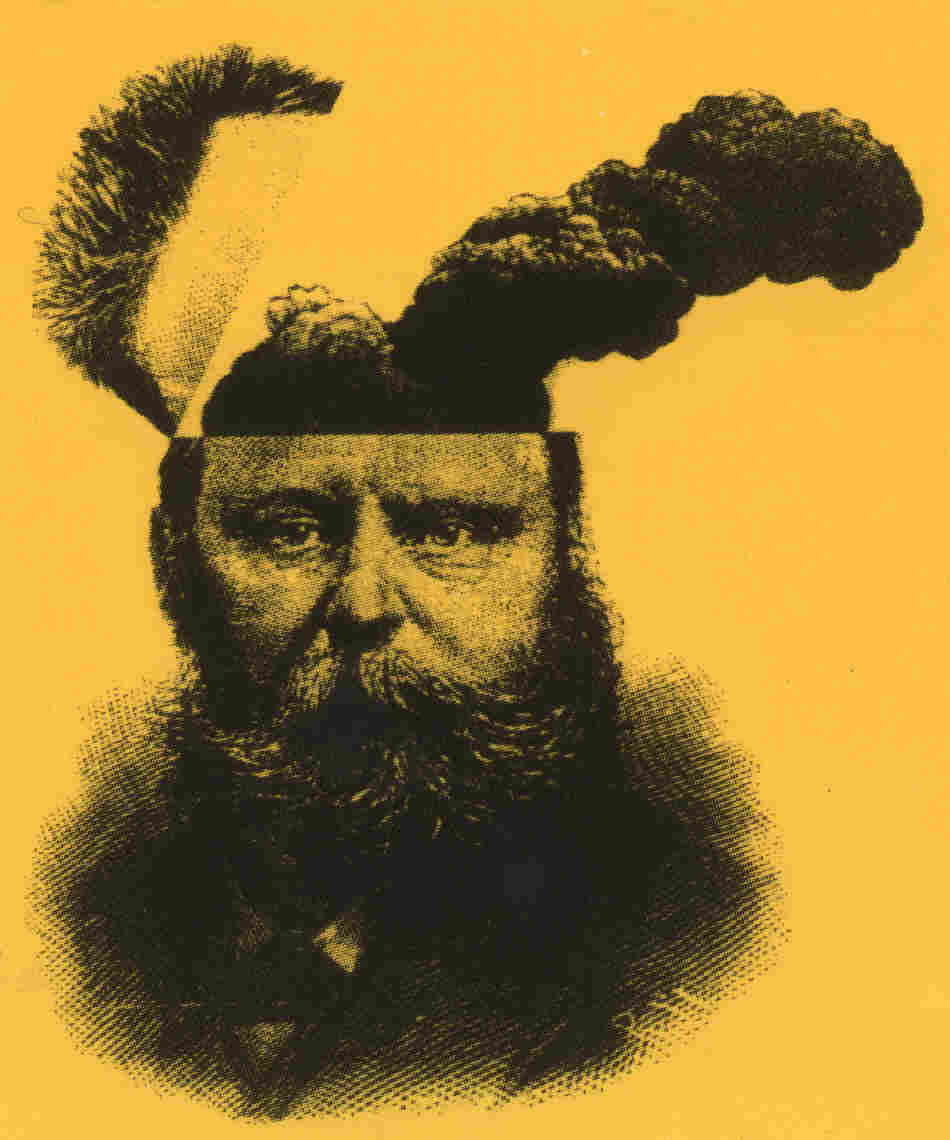
\includegraphics[width=0.3\linewidth]{mindblown.jpg}
 \end{figure}
Magenta doesn't exist in nature. It is trick our brains and cameras
play on us. It exists because we sample the spectrum and try to
recombine the samples. We wrap the visible spectrum around. 
\end{frame}
% ------------------------------------------------
\begin{frame}
\frametitle{To manage this problem we use color spaces.}
 \begin{figure}
     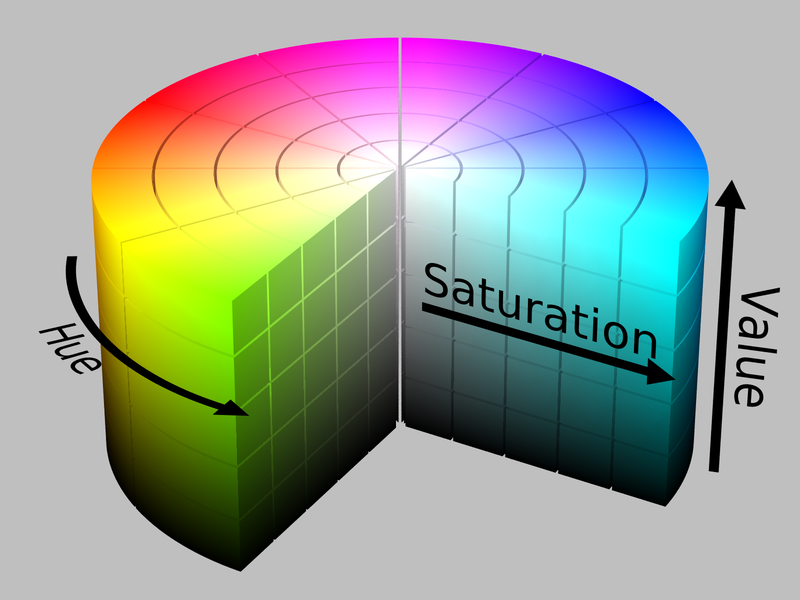
\includegraphics[width=0.4\linewidth]{hsv.png}
 \end{figure}
\begin{itemize}
\item To deal with this problem we use color spaces. 
\item Most images are in the RGB, BGR, or gray scale color spaces.
\item Sometimes it is helpful to use the hue, saturation, and value (HSV)
color space. In HSV you have a 
\begin{itemize}
\item Hue, or pure color (from 0 to 180) 
\item Saturation that tells us how far from white our color is
\item Value that tells us how dark the color is.
\end{itemize}
\end{itemize}
\end{frame}


% ------------------------------------------------
\begin{frame}
\frametitle{How do I work with Color in SimpleCV}
\begin{itemize}
\item The \textbf{Image.toHSV()} function will convert your image, while the
\textbf{Image.toBGR()} function will return it back to the original.
\item We also have \textbf{Image.toGray()} and \textbf{Image.toRGB()}
  and whole bunch more. 
\item The \textbf{Image.huePeaks} function can help you guess what
  hues are in your image.
\item The \textbf{Image.hueDistance} function can then help you look
  for stuff that is the hue you want. 
\item The \textbf{Image.hueHistogram} function will let you visualize
  the results. 
\end{itemize}
\end{frame}
% ------------------------------------------------
\begin{frame}[fragile] 
\frametitle{Finding colors}
\begin{example}[Using Hue]
\begin{minted}[fontsize=\tiny]{python}
import pylab as plt # import pylab for plotting
img = Image("flower.jpg")
img.show()
peaks = img.huePeaks() # find the hues
print peaks
hist = img.hueHistogram() # get the histogram too
plt.plot(hist) # plot the histogram
plt.draw() # show it to us
# show how far away from the hue we are black is closer
# white is farther away from our hue.
hdist = img.hueDistance(peaks[3][0]) 
# create a black and white version of our flower
binary = img.hueDistance(peaks[3][0]).invert().threshold(220)
hdist.show()
binary.show()
hdist.save('hflower.png')
binary.save('bflower.png')
\end{minted}
\end{example}
\end{frame}
% ------------------------------------------------
\begin{frame}
\frametitle{Color Finding Results}
 \begin{figure}
     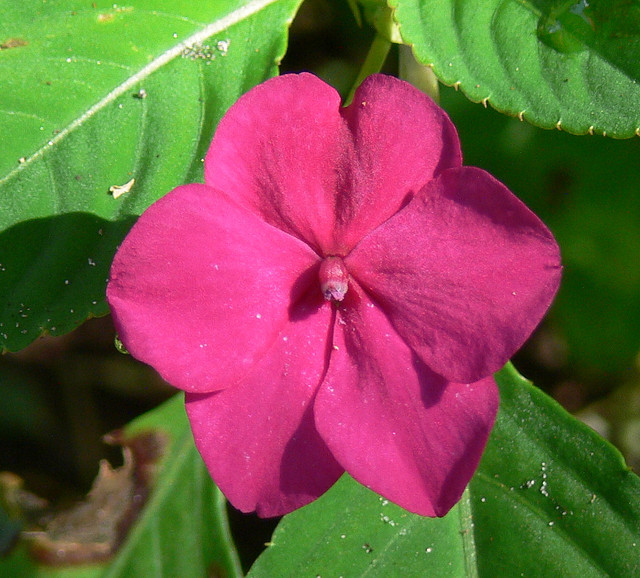
\includegraphics[width=0.3\linewidth]{flower.jpg}
     \quad
     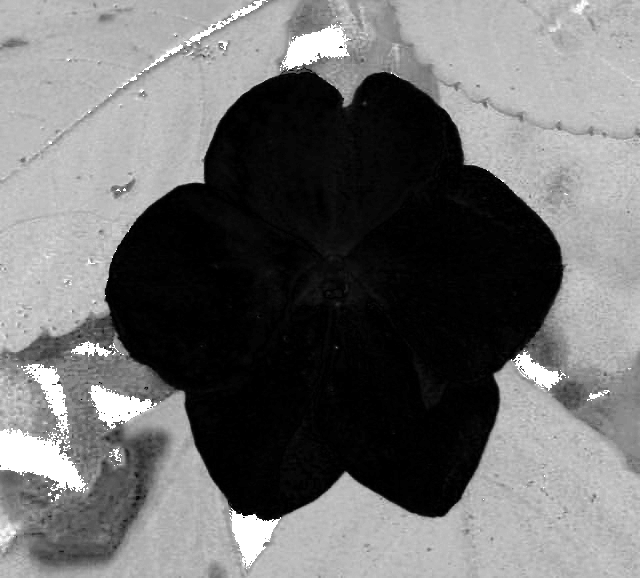
\includegraphics[width=0.3\linewidth]{hflower.png}
     \quad
     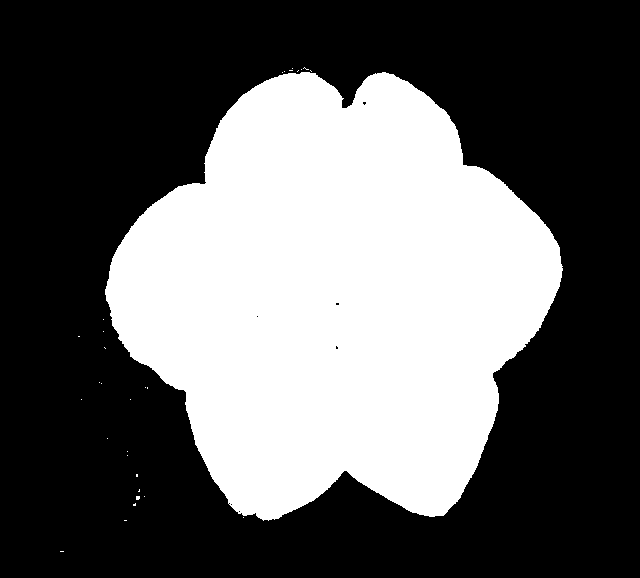
\includegraphics[width=0.3\linewidth]{bflower.png}
     \quad
     \caption{Finding an object from colors}
 \end{figure}
\end{frame}

% -----------------------------------------------
\begin{frame}
\frametitle{How do I work \textbf{without}  Color in SimpleCV}
Color is not so important when all we care about are light or dark
things. 
\begin{itemize}
\item We can use the \textbf{Image.toGray} method to create gray
  images. Gray pixels only go from values of 0 to 255
\item Sometimes it is helpful to adjust the contrast for us to find objects.
  \begin{itemize}
    \item If the gray values in our image only go from say [50,150] we
      can us the \textbf{Image.equalize} method to interpolate them to
      values between [0,255].
    \item Other times we want to enhance a certain space of the gray
      spectrum. We can use the \textbf{Image.stretch} function. 
    \end{itemize}
\item \textbf{Image.histogram} can help us figure out what gray values
  are present.
\item \textbf{Image.maxVal} and \textbf{Image.minVal} can help us
  determine the range of intensities and where to set our thresholds.
\end{itemize}
\end{frame}
% ------------------------------------------------
\begin{frame}[fragile] 
\frametitle{Shades of Gray}
\begin{example}[Modify Grayscale Images]
\begin{minted}[fontsize=\small]{python}
img = Image('penguins.jpg')
img = img.toGray()
eImg = img.crop(180,400,100,100)
img.drawRectangle(180,400,100,100)
plt.plot(eImg.histogram(), '-r')
plt.plot(eImg.equalize().histogram(),'-b')
plt.show()
img.show()
eImg.show()
eImg.equalize().show()
max = eImg.maxValue()
min = eImg.minValue()
print [max, min]
streched = img.stretch(min,max)
streched.show()
\end{minted}
\end{example}
\end{frame}
% -----------------------------------------------
\begin{frame}
\frametitle{Seeing in Black and White - Binary Images}
\small{Very often we want to just isolate a certain area in an image and mark
it. To do this we use binary images, also called masks. The general
process of creating a binary image is called segmentation. Often we call
the white areas foreground and the black areas background. }
\begin{itemize}
\item We can use the\textbf{Image.threshold} method to create a binary
  image. 
  \begin{itemize}
  \item Threshold will set gray values below the threshold to black
    and areas above the threshold to white.
  \item SimpleCV will automatically convert color images to grayscale
    images for a threshold.
  \end{itemize}
\item The \textbf{Image.binarize} method will also create a binary
  image.
   \begin{itemize}
   \item Binarize uses Otsu's method which changes the threshold
     automatically to improve performance. 
   \item There are a lot of parameters to tweak so checkout the
     documentation.
  \end{itemize}
\end{itemize}
\end{frame}

% ------------------------------------------------
\begin{frame}[fragile] 
\frametitle{Basic Binarization}
\begin{example}[Let's find the parrot]
\begin{minted}[fontsize=\small]{python}
img = Image('parrot.jpg')
b = img.binarize().invert() # automatic
t1 = img.threshold(50) # too low
t2 = img.threshold(128) # okay
t3 = img.threshold(200) # too high
b.show()
t1.show()
t2.show()
t3.show()
b.save('bparrot.png')
t1.save('t1parrot.png')
t2.save('t2parrot.png')
t2.save('t3parrot.png')
\end{minted}
\end{example}
\end{frame}
% ------------------------------------------------
\begin{frame}
\frametitle{Binzarization Results}
 \begin{figure}
     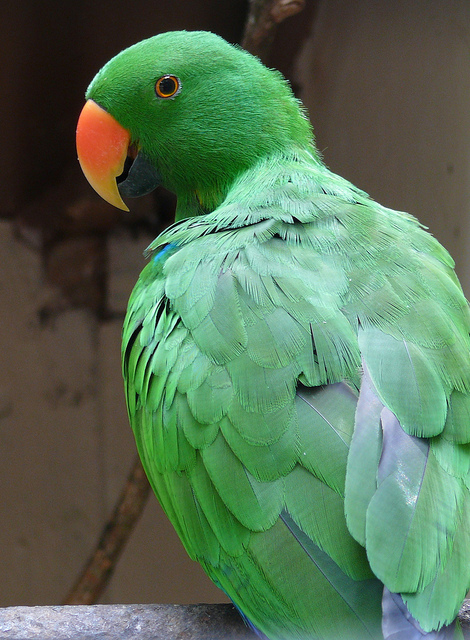
\includegraphics[width=0.15\linewidth]{parrot.jpg}
     \quad
     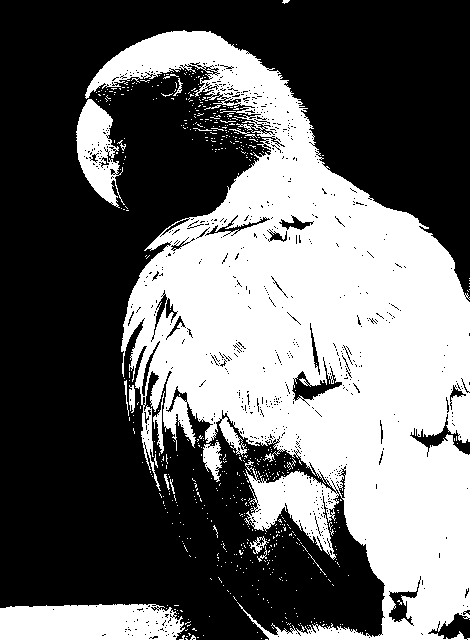
\includegraphics[width=0.15\linewidth]{bparrot.png}
     \quad
     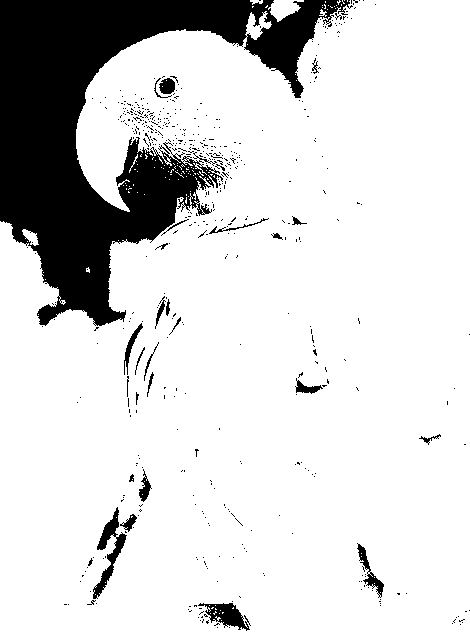
\includegraphics[width=0.15\linewidth]{t1parrot.png}
     \quad
     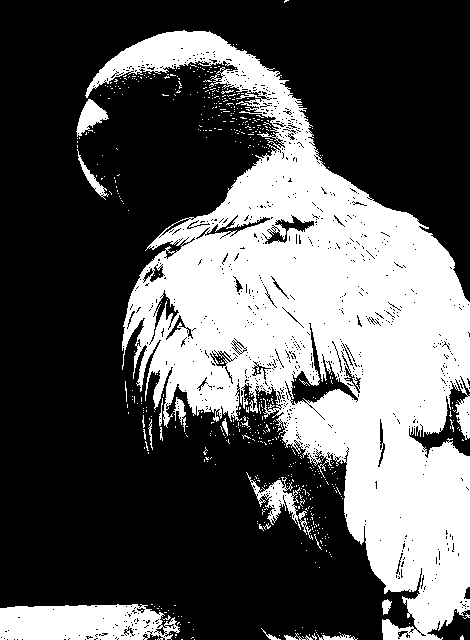
\includegraphics[width=0.15\linewidth]{t2parrot.png}
     \quad
     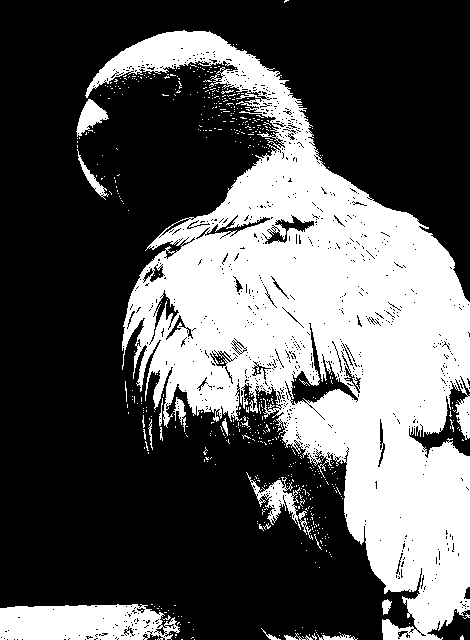
\includegraphics[width=0.15\linewidth]{t3parrot.png}
 \end{figure}
Left to right, source image, binarize using Otsu's method, threshold =
50, threshold=128, threshold=200
\end{frame}
% -----------------------------------------------
\begin{frame}
  \frametitle{Morphological Operations - Fixing Binarized Images}
 \begin{figure}
     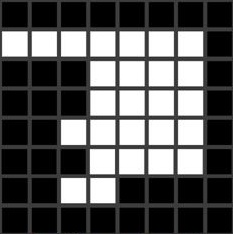
\includegraphics[width=0.1\linewidth]{morph-src.jpg}
     \quad
     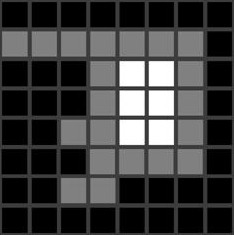
\includegraphics[width=0.1\linewidth]{morph-erode.jpg}
     \quad
     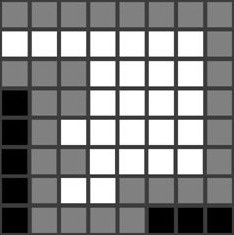
\includegraphics[width=0.1\linewidth]{morph-dilate.jpg}
     \caption{Source image, source after erosion, source after dilation.}
 \end{figure}

We can clean up binary images using basic morphology operations.
\begin{itemize}
\item We can use the\textbf{Image.dilate} to enlarges our white areasand
  connects them.
  \begin{itemize}
  \item Basically if a pixel touches a white pixel we set it to white.
  \item Can be used repeatedly. Works in color too.
  \end{itemize}
\item The \textbf{Image.erode} method shrinks our white areas
  image.
   \begin{itemize}
   \item If a white pixel touches a black pixel we set it to black.
   \item Can be used repeatedly.
  \end{itemize}
\item \textbf{Image.morphOpen} and \textbf{Image.morphClose} do
  similar things but are used to open and close regions.
\end{itemize}
\end{frame}
% -----------------------------------------------
\begin{frame}
  \frametitle{Fixing Binarized Images II }

There are other techniques we can use to fix things. 
\begin{itemize}
\item \textbf{Image.floodFill} works just like the paint bucket tool
  in an image editor. It can get rid of areas.
\item \textbf{Image.watershed} is a sophisticated technique that can
  really help.
\item We can also logically and, or, xor, and nand images. 
  \begin{itemize}
  \item Logical and is just multiplication or \textbf{Image.logicalAND} 
  \item Logical or is just multiplication or \textbf{Image.logicalOR} 
  \item Logical xor is \textbf{Image.logicalXOR} 
  \item Logical nand is \textbf{Image.logicalNAND}
  \item These all work in color and gray scale too.
  \end{itemize}
\end{itemize}
\end{frame}
% ------------------------------------------------
\begin{frame}[fragile] 
\frametitle{Advanced Binarization}
\begin{example}[Get a binary representation of the parrot.]
\begin{minted}[fontsize=\small]{python}
img = Image('parrot.jpg')
img.show()
binary = img.binarize().invert() # automatic
binary.show() # good but we're missing part of the beak
binary2 = img.hueDistance(80).invert().threshold(190)
binary2.show() # missing a different part of the beak
filled = binary.floodFill((0,img.height-1),color=Color.BLACK)
filled.show() # get rid of the branch in the corner
better = filled.logicalOR(binary2)
better.show() # combine the two.
eroded = better.erode()
eroded.show() # get rid of specs.
dilated = better.dilate()
dilated.show() # get rid of holes
watershed = img.watershed(dilated)
watershed.show() # let's see what this can do
\end{minted}
\end{example}
\end{frame}

%binary.save('mbparrot.png')
%binary2.save('mb2parrot.png')
%filled.save('filledparrot.png')
%better.save('betterparrot.png')
%eroded.save('erodeparrot.png')
%dilated.save('dilatedparrot.png')
%watershed.save('watershedparrot.png')

% ------------------------------------------------
\begin{frame}
\frametitle{Parrot Pipeline}
 \begin{figure}
     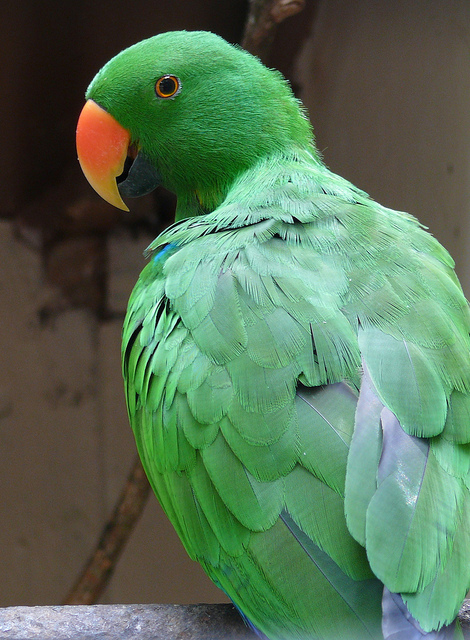
\includegraphics[width=0.15\linewidth]{parrot.jpg}
     \quad
     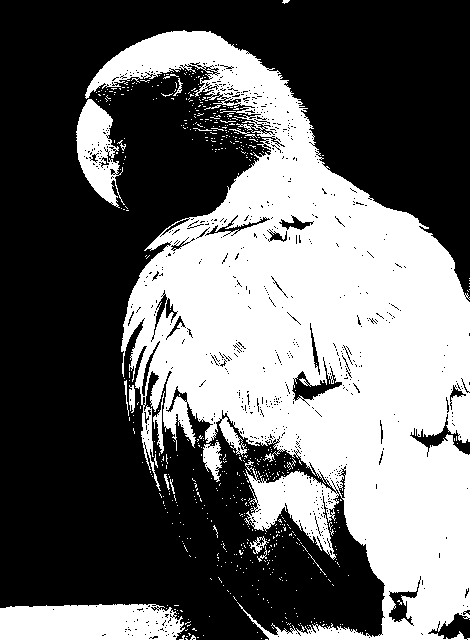
\includegraphics[width=0.15\linewidth]{mbparrot.png}
     \quad
     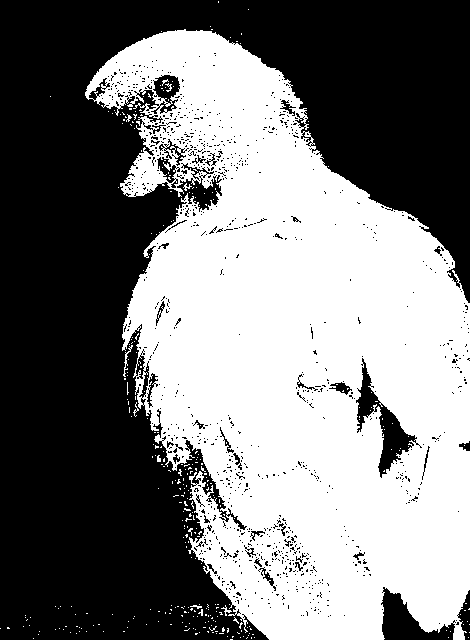
\includegraphics[width=0.15\linewidth]{mb2parrot.png}
     \quad
     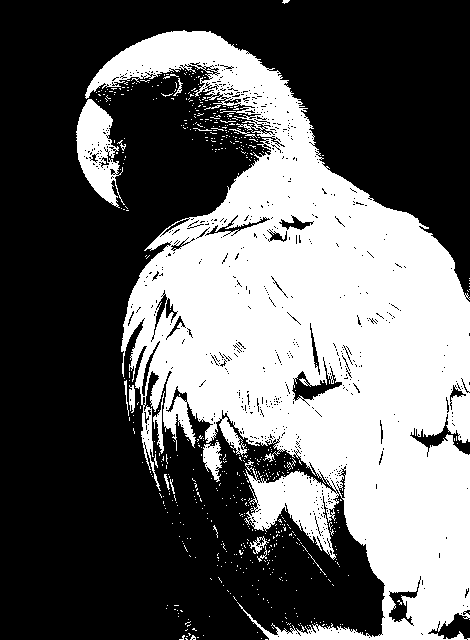
\includegraphics[width=0.15\linewidth]{filledparrot.png}
 \end{figure}
 \begin{figure}
     \includegraphics[width=0.15\linewidth]{betterparrot.png}
     \quad
     \includegraphics[width=0.15\linewidth]{erodeparrot.png}
     \quad
     \includegraphics[width=0.15\linewidth]{dilatedparrot.png}
     \quad
     \includegraphics[width=0.15\linewidth]{watershedparrot.png}
 \end{figure}

\tiny{Or pipeline, left to right, top to bottom}
\end{frame}

% ------------------------------------------------
% ------------------------------------------------
% ------------------------------------------------
\section{Finding Stuff}

% ------------------------------------------------
% ------------------------------------------------
% ------------------------------------------------

\begin{frame}
  \frametitle{Finding Stuff}
 \begin{figure}
     \includegraphics[width=0.2\linewidth]{waldo.jpg}
 \end{figure}

Now that we've got a lot of the basics down let's start doing stuff
with images. Let's \textbf{find} interesting sets of \textbf{features} in our images.

\end{frame}
% ------------------------------------------------
\begin{frame}
  \frametitle{Finding Stuff II}

SimpleCV allows you to quickly and easily find \textbf{features} in
your images using a variety of methods that begin with the word
\textbf{find}. 
\\~\\
\textbf{Features} have a set of basic properties that makes
manipulating them super easy.
\\~\\
The \textbf{Image.findXXXX} methods each return a \textbf{FeatureSet}
which is a list of features.
\\~\\
A \textbf{FeatureSet} also allows you to look at aggregate information
about features.
\end{frame}
% ------------------------------------------------
\begin{frame}
  \frametitle{Things you can find in SimpleCV}

  \begin{columns}[c] % The "c" option specifies centered vertical alignment while the "t" option is used for top vertical alignment

    \column{.5\textwidth} % Left column and width
    \begin{itemize}
    \item Blobs - binary objects
    \item Lines
    \item Corners
    \item Circles
    \item Haar Features
      \begin{itemize}
        \item faces
        \item eyes
        \item mouths
        \item much more.
        \end{itemize}
    \end{itemize}

    \column{.5\textwidth} % Left column and width
    \begin{itemize}
    \item Barcodes
    \item Text
    \item Templates (example images)
    \item Keypoints (interesting areas)
    \item Keypoint Matches
    \item Motion (between images)
    \item Skintone Blobs
    \end{itemize}

  \end{columns}
\end{frame}
% ------------------------------------------------
\begin{frame}
  \frametitle{The Basic Mechanics}

Once you have a \textbf{FeatureSet} you can use iteration either in a
loop or using python list comprehensions to filter your features to
get what you want. 
\begin{itemize}
\item \textbf{Feature.draw} Will draw the feature on the source image.
\item \textbf{Feature.show} Will show the feature on the source image.
\item \textbf{Feature.crop} Will return an image of just the feature.
\item \textbf{Feature.meanColor} Will return the average color. 
\item The feature's width, height, and position can also be checked.
\end{itemize}
\end{frame}
% ------------------------------------------------
\begin{frame}
  \frametitle{The Basic Mechanics II}

\begin{itemize}
\item \textbf{Feature.area} gives the area of the feature.
\item \textbf{FeatureSet.filter} Allows you to filter features on
  different criteria.
\item \textbf{FeatureSet.distanceFrom} will return the distance of
  each feature from a point.
\item \textbf{FeatureSet.area} returns the area of every feature as a
  list. By default we sort the feature set from smallest to largest.
\item FeaturesSets also know the center points of the features and
  their corners. 
\end{itemize}
\end{frame}

% ------------------------------------------------
\subsection{blobs}
% ------------------------------------------------
\begin{frame}
  \frametitle{Finding Blobs}

\textbf{Blob} is a backronym for binary large object. They are
basically anything that would be white in a binary image. You can find
blobs in a variety of ways:
\begin{itemize}
\item \textbf{Image.findBlobs} will do a binarize and return the blobs
  it found.
\item \textbf{Image.findBlobs} will use a binary image, also called a
  masks, to find blobs.
\item \textbf{Image.findBlobsFromPalette} will find blobs with
  specific colors from a palette
\item \textbf{Image.findBlobsFromWatershed} will find blobs using the
  watershed algorithm and a binary image you provide
\end{itemize}
\end{frame}
% ------------------------------------------------
\begin{frame}
  \frametitle{Let's see an example.}
 \begin{figure}
     \includegraphics[width=0.7\linewidth]{cookies.jpg}
 \end{figure}
Can we write some python to find the star cookie in the top right corner?
\end{frame}
% ------------------------------------------------
\begin{frame}[fragile] 
\frametitle{Sorting blobs}
\begin{example}[Finding the yellow cookie in the corner.]
\begin{minted}[fontsize=\tiny]{python}
img = Image('cookies.jpg')
# find our cookes and draw them red, filled in
blobs = img.findBlobs(threshval=128, minsize=200)
blobs.draw(width=-1, color=Color.RED) #autocolor= True)
# find the mean and std blob areas
areaAvg = np.mean(blobs.area())
areaStd = np.std(blobs.area())
# filter the cookies by area and draw those green
lilcookies = blobs.filter(blobs.area() < areaAvg+2.5*areaStd  )
lilcookies.draw(width=-1,color=Color.GREEN)
# Now sort the cookies so the yellow ones are at at 0
lilcookies = lilcookies.sortColorDistance(color=Color.YELLOW)
lilcookies[0:4].draw(width=-1,color=Color.YELLOW)
# Now take our yellow cookies and see how
# far they are away from the top right corner
dists = lilcookies[0:4].distanceFrom((img.width,0))
# find the closest one to the corner
location = np.where(dists==np.min(dists))[0][0]
lilcookies[location].crop().show()
lilcookies[location].draw(width=-1,color=Color.HOTPINK)
img.show()
\end{minted}
\end{example}
\end{frame} 
% ------------------------------------------------
\begin{frame}
\frametitle{Cookie Sorting}
 \begin{figure}
     \includegraphics[width=0.3\linewidth]{cookies.jpg}
     \quad
     \includegraphics[width=0.3\linewidth]{foundblobs.png}
     \quad
     \includegraphics[width=0.3\linewidth]{foundsmallblobs.png}
 \end{figure}
 \begin{figure}
     \includegraphics[width=0.3\linewidth]{yellowblobs.png}
     \quad
     \includegraphics[width=0.3\linewidth]{pinkblobs.png}
 \end{figure}
\end{frame}
% ------------------------------------------------
\begin{frame}
  \frametitle{Advanced Blobs}
Blobs have a low other neat features.
\begin{itemize}
\item \textbf{Blob.minRect} The rotated rectangle that best encloses
  the blobs.
\item \textbf{Blob.contour} A list of (x,y) tuples and other lists of
  (x,y) tuples that describe the outer contour.
\item \textbf{Blob.hull} The contour of the blob if you were
  to stretch a rubber band around it. This eliminates what we call
  concavities.
\item \textit{Blob.mHoleContour} gives a list of the holes and
  ``islands'' in the holes of the blob. This is a list of list that
  may have lists inside of them. 
\end{itemize}
\end{frame}
% ------------------------------------------------
\begin{frame}
  \frametitle{Advanced Blobs II}
Blobs have a lot of other neat features.
\begin{itemize}
\item \textbf{Blob.drawRect} Draw the square region around the blob.
\item \textbf{Blob.drawMinRect} Draw the minimum bounding rectangle
  for each blob.
\item \textbf{Blob.drawOutline} The outline of the blob without the holes.
  may have lists inside of them. 
\item \textbf{Blob.drawHoles} Draw just the holes. 
\item \textbf{Blob.drawHull} Draw just the blob's convex hull. (The
  rubber band version.)
\item \textit{These are order dependent! They can overwrite each other}
\end{itemize}
\end{frame}
% ------------------------------------------------
\begin{frame}[fragile] 
\frametitle{Blob drawing in action!}
  \frametitle{Let's see an example.}
 \begin{figure}
     \includegraphics[width=0.3\linewidth]{handblob.png}
 \end{figure}
\begin{example}
\begin{minted}[fontsize=\tiny]{python}
img = Image('hand.jpg')
blobs = img.findBlobs(minsize=200)
blob = blobs[0]
blob.drawHull(color=Color.HOTPINK,width=4)
blob.draw(color=Color.RED,width=2)
blob.drawRect(color=Color.GREEN, width=4)
blob.drawMinRect(color=Color.BLUE, width=4)
blob.drawHoles(color=Color.YELLOW, width=-1)
img.show()
img.applyLayers().save('handblob.png')
\end{minted}
\end{example}
\end{frame}

% ------------------------------------------------
\begin{frame}
  \frametitle{Advanced Blobs III - Masks}
Sometimes we want to work with binary image that comes from a blob.
\begin{itemize}
\item \textbf{Blob.blobImage} An image of just the blob region.
\item \textbf{Blob.hullImage} An image of just the blob's hull region.
\item \textbf{Blob.blobMask} A binary image of just the blob.
\item \textbf{Blob.hullMask} A binary image of the blob's convex hull.
\item \textbf{Blob.getFullMaskedImage} Get the original image with
  everything black except for the blob. There is also a convex hull version.
\item \textbf{Blob.getFullMask} Get the original sized as a binary
  mask of the blob. Also has a hull variant.
\item \textbf{Blob.getEdgeImage} return an image of just the blobs
  outer edge. Also has full and hull variants. 
\end{itemize}
\end{frame}
% ------------------------------------------------
\begin{frame}[fragile] 
\frametitle{Masks, Edges, etc}
\begin{example}
\begin{minted}[fontsize=\tiny]{python}
img = Image('albino.jpg')
img.show()
blobs = img.findBlobs(minsize=200)
blob = blobs[-1]
src = blob.mImg
src = src.sideBySide(blob.blobImage())
src = src.sideBySide(blob.hullImage())
src = src.sideBySide(blob.blobMask())
src = src.sideBySide(blob.hullMask())
src = src.sideBySide(blob.getEdgeImage())
src = src.sideBySide(blob.getHullEdgeImage())
src = src.scale(0.5)
src.show()
src.save('albinoblob.png')
big = img
big = big.sideBySide(blob.getFullMaskedImage())
big = big.sideBySide(blob.getFullHullMaskedImage())
big = big.sideBySide(blob.getFullMask())
big = big.sideBySide(blob.getFullEdgeImage())
big = big.sideBySide(blob.getFullHullEdgeImage())
big = big.scale(0.3)
big.show()
big.save('albinoimgs.png')
\end{minted}
\end{example}
\end{frame}
% ------------------------------------------------
\begin{frame}
\frametitle{Comparing Mask Options}
 \begin{figure}
     \includegraphics[width=0.9\linewidth]{albinoblob.png}
 \end{figure}
 \begin{figure}
     \includegraphics[width=0.9\linewidth]{albinoimgs.png}
 \end{figure}
\end{frame}
% ------------------------------------------------
\begin{frame}
  \frametitle{Advanced Blobs IV - Shape}
We can use shape information to compare blobs
\begin{itemize}
\item \textbf{Blob.area} The total number of pixels in the blob.
\item \textbf{Blob.perimeter} The length of the outside of the blob.
\item ProTip the area/perimeter is a nice metric for smoothness.
\item \textbf{Blob.angle} The angle between the minimum rectangle and
  horizontal in degrees. 
\item \textbf{Blob.centroid} The center of mass, not the center of the
  bounding box.
\item \textbf{Blob.rotate} Rotate a blob a certain number of
  degrees. This changes the blobs internal state. 

\end{itemize}
\end{frame}

% ------------------------------------------------
\begin{frame}
  \frametitle{Advanced Blobs V - Shape}
We can use shape information to compare blobs
\begin{itemize}
\item \textbf{Blob.circleDistance} and \textbf{Blob.isCircle} help to
  find circular things.
\item \textbf{Blob.rectangleDistance} and \textbf{Blob.isRectangle} help to
  find rectangular things
\item \textbf{Blob.isSquare} returns true if a blob is squareish. 
\item \textit{Blob.mHu} A list of the seven Hu moments. These are like
  moments of inertia in physics. Hu moments don't care about
  rotation, and they are really helpful for matching blobs
\item \textbf{Blob.match} returns a match value against a particular
  blob based on shape using Hu moments.
\end{itemize}
\end{frame}
% ------------------------------------------------
\begin{frame}[fragile] 
\frametitle{Matching blobs}
\begin{example}[Try to find the horse cookies given a template.]
\begin{minted}[fontsize=\tiny]{python}
img = Image('cookies.jpg')
# find our cookes and draw them red, filled in
blobs = img.findBlobs(threshval=128, minsize=200)
blobs.draw(width=-1, color=Color.RED) #autocolor= True)
# find the mean and std blob areas
areaAvg = np.mean(blobs.area())
areaStd = np.std(blobs.area())
# filter the cookies by area and draw those green
lilcookies = blobs.filter(blobs.area() < areaAvg+2.5*areaStd  )
lilcookies.draw(width=-1,color=Color.GREEN)
# Now sort the cookies so the yellow ones are at at 0
lilcookies = lilcookies.sortColorDistance(color=Color.YELLOW)
lilcookies[0:4].draw(width=-1,color=Color.YELLOW)
# Now take our yellow cookies and see how
# far they are away from the top right corner
dists = lilcookies[0:4].distanceFrom((img.width,0))
# find the closest one to the corner
location = np.where(dists==np.min(dists))[0][0]
lilcookies[location].crop().show()
lilcookies[location].draw(width=-1,color=Color.HOTPINK)
img.show()
\end{minted}
\end{example}
\end{frame} 
% ------------------------------------------------
\begin{frame}
\frametitle{Cookie Matching Results}
 \begin{figure}
     \includegraphics[width=0.7\linewidth]{matchingblobs.png}
 \end{figure}
\end{frame}
% ------------------------------------------------
\subsection{Finding Lines}
% ------------------------------------------------
\begin{frame}
  \frametitle{Finding Lines}
SimpleCV makes it easy to find straight lines.
\begin{itemize}
\item \textbf{Image.edges} creates an image of all the lines in the
  image using the Canny edge detector.
\item There are two thresholds that you can tweak to improve
  performance. 
\item \textbf{Image.findLines} will apply the Canny edge detector and
  then use the Hough transform to find the straight lines.
\item \textbf{Image.findLines} returns a FeatureSet of Line features
  that you can then filter.
\end{itemize}
\end{frame}

% ------------------------------------------------
\begin{frame}
  \frametitle{The Line Feature}
\begin{itemize}
\item The line feature can be found in Detection.py
\item Each line knows its length, its average color, its angle.
\item \textbf{Line.findIntersection} can be used to find line intersections.
\item You can also test for parallel and perpendicular lines
\end{itemize}
\end{frame}
% ------------------------------------------------
% ------------------------------------------------
\begin{frame}[fragile] 
\frametitle{Line Finding Example}
\begin{example}
\begin{minted}[fontsize=\small]{python}
img = Image('hallway.jpg')
img.show()
img.edges().show()
img.edges().save('hallwayedges.png')
lines = img.findLines() # get the lines
# return only long ones
lines = lines.filter(lines.length() > 50 )
lines.show(width=3)
# now find the horz and vert lines by 
# filtering on the angle.
vertical = lines.filter((np.abs(lines.angle()) > 80))
horizontal = lines.filter(np.abs(lines.angle()) < 10 )
vertical.draw(width=3,color=Color.RED)
horizontal.draw(width=3,color=Color.BLUE)
img.show()
img.applyLayers().save('hallwaylines.png')
\end{minted}
\end{example}
\end{frame} 
% ------------------------------------------------
\begin{frame}
\frametitle{Line find results.}
 \begin{figure}
     \includegraphics[width=0.4\linewidth]{hallway.jpg}
     \quad
     \includegraphics[width=0.4\linewidth]{hallwayedges.png}
 \end{figure}
 \begin{figure}
     \includegraphics[width=0.4\linewidth]{hallwaylines.png}
 \end{figure}
\end{frame}
% ------------------------------------------------
% ------------------------------------------------
\subsection{Finding Circles}
% ------------------------------------------------
\begin{frame}
  \frametitle{Finding Circles}
SimpleCV makes it easy to find circles too.
\begin{itemize}
\item Just like before we use the edge image. 
\item \textbf{Image.findCircle} returns a FeatureSet of Circle features
  that you can then filter.
\item There are three thresholds that you can tweak to improve
  performance. One for the edges, one for the circle detector, and one
  for the circle spacing.
\item  Circle features have all of the usual features like mean color
  along with the ones you would expect like radius, diameter, etc. 
\end{itemize}
\end{frame}
% ------------------------------------------------
% ------------------------------------------------
\begin{frame}[fragile] 
\frametitle{Line Finding Example}
\begin{example}
\begin{minted}[fontsize=\tiny]{python}

\end{minted}
\end{example}
\end{frame} 
% ------------------------------------------------
\begin{frame}
\frametitle{Line find results.}
 \begin{figure}
     \includegraphics[width=0.4\linewidth]{hallway.jpg}
     \quad
     \includegraphics[width=0.4\linewidth]{hallwayedges.png}
 \end{figure}
 \begin{figure}
     \includegraphics[width=0.4\linewidth]{hallwaylines.png}
 \end{figure}
\end{frame}
% ------------------------------------------------
% ------------------------------------------------
\subsection{Finding Templates}
% ------------------------------------------------
\begin{frame}
  \frametitle{Template Matching}
Sometimes you have an image that you want to use as a ``template'' and you
want to match it to something in your image. 
\begin{itemize}
\item \textbf{Image.findTemplate} returns a FeatureSet of template features
  that you can then filter.
\item Templates can handle a little bit of rotation, illumination
  change, and skew, but not much.
\item you can try slightly rotating your template, or using the edge
  image of something like the \textbf{Image.sobel} operation to
  improve performance.
\item The performance of the matching can be tuned using different
  matching methods and by tweaking the threshold.
\end{itemize}
\end{frame}
% ------------------------------------------------
% ------------------------------------------------
\begin{frame}[fragile] 
\frametitle{Template Finding Example}
\begin{example}
\begin{minted}[fontsize=\small]{python}
img = Image('coins1.jpg')
mask = img.threshold(130).invert()
blobs = img.findBlobsFromMask(mask, minsize=200)
blobs.show(width=-1)
img.clearLayers()
blobs[-5].crop().show()
template = blobs[-5].crop()
template.save('template1.png')
found = img.findTemplate(template,threshold=2.2)
found.draw(color=Color.RED)
template2 = blobs[5].crop()
template2.save('template2.png')
template2.show()
found2 = img.findTemplate(blobs[5].crop(),threshold=4.15)
found2.draw(color=Color.BLUE)
found2.show()
img.save('foundtemplates.png')
\end{minted}
\end{example}
\end{frame} 
% ------------------------------------------------
\begin{frame}
\frametitle{Template finding results.}
 \begin{figure}
     \includegraphics[width=0.4\linewidth]{foundtemplates.png}
 \end{figure}
 \begin{figure}
     \includegraphics[width=0.1\linewidth]{template1.png}
     \quad
     \includegraphics[width=0.1\linewidth]{template2.png}
 \end{figure}
\end{frame}
% ------------------------------------------------
% ------------------------------------------------
\subsection{Finding Motion}
% ------------------------------------------------
\begin{frame}
  \frametitle{Motion Finding}
Another common task is looking for motion. If you just want to detect
change looking at the difference between images usually
suffices. However sometimes you want to know more.
\begin{itemize}
\item \textbf{Image.findMotion} returns a FeatureSet of motion values
  between two images.
\item This method takes in a second image and then reports the
  motion. The image sizes must match. 
\item SimpleCV uses an algorithm called optical flow of which there
  are several variants. You can pick the one that works best for you.
\item There is one parameter to tweak, called window, which is the
  sample window size. Faster movement requires larger windows.
 
\end{itemize}
\end{frame}
% ------------------------------------------------
\begin{frame}
  \frametitle{Motion Finding II}
\begin{itemize}
\item The images should have a reasonable amount of edges, and be
  fairly close together in time. 
\item Motion will be most obvious around strong edges, less so
around plain areas, but some false positives tend to happen.
\item By default the rendered motion is scaled to unit length, but the
  actual values vary considerably.  
\item Be aware that there is motion from the camera, and motion from
objects moving. 
\item Works a lot better on a live camera.
\item The algorithms can be computationally beefy, scale images to get
  better results. 
\end{itemize}
\end{frame}
% ------------------------------------------------
\begin{frame}[fragile] 
\frametitle{Motion Finding Example I}
\begin{example}
\begin{minted}[fontsize=\small]{python}
img1 = Image('toys1.jpg')
img1 = img1.scale(0.5)
img1.show()
img2 = Image('toys2.jpg')
img2 = img2.scale(0.5)
img2.show()
motion = img2.findMotion(img1,method="BM",window=27)
motion.show(width=3)
img2.clearLayers()
mags = [m.magnitude() for m in motion]
bigMove = motion.filter( mags > np.mean(mags))
bigMove.show(color=Color.RED, width=3)
bigMove.applyLayers().save('motion.png')
\end{minted}
\end{example}
\end{frame} 
% ------------------------------------------------
\begin{frame}
\frametitle{Motion finding results.}
 \begin{figure}
     \includegraphics[width=0.7\linewidth]{motion.png}
 \end{figure}
\end{frame}
% ------------------------------------------------
\begin{frame}[fragile] 
\frametitle{Motion Finding Example II}
This works a lot better as a live example. 
\begin{example}[MotionExample.py]
 \inputminted[linenos=true, tabsize=4,
 fontsize=\tiny]{python}{MotionExample.py}
\end{example}
\end{frame} 
% ------------------------------------------------
\subsection{Optional Libs - Text and Barcodes.}
% ------------------------------------------------
\begin{frame}
  \frametitle{Finding Text and Reading Barcodes}
Text and barcode reading are optional libraries that we've added hooks
for. 
\begin{itemize}
\item \textbf{Image.findBarcodes} uses either lib zxing or zlib. 
  \begin{itemize}
    \item Each has its advantages and disadvantages. Generally zxing works better.
    \item Returns a barcode feature with the location and the data. 
  \end{itemize}
\item \textbf{Image.readText} uses python bindings to the tesseract
  library.
  \begin{itemize}
    \item Does not work in the SimpleCV ipython notebook, but we're
      working on it. 
   \item Translation to string often leaves lots of spare
     characters. Formatting is an issue. 
  \end{itemize}
\end{itemize}
\end{frame}
% ------------------------------------------------
\begin{frame}[fragile] 
\frametitle{Reading a QR Code}
\begin{example}
\begin{minted}[fontsize=\small]{python}
qrimg = Image('qrcode.png')
qrimg.show()
bc = qrimg.findBarcode()
bc.show(width=3)
print bc[0].data
qrimg.drawText(str(bc[0].data),10,10, \\
               color=Color.RED,fontsize=24)
qrimg.show()
img = Image('textcard.jpg')
img.show()
print img.readText()
\end{minted}
\end{example}
\end{frame} 
\subsection{Finding Faces and Face Features}
% ------------------------------------------------
\begin{frame}
  \frametitle{Face Finding}
There are built in utilities in SimpleCV for finding faces and parts
of faces.
\begin{itemize}
\item These parts of the face are found using what is called a Haar
  Cascade. 
\item Lots of data and research went into developing these tools. 
\item \textbf{Image.findHaarFeatures} returns a FeatureSet of features
  corresponding to the cascade you pass it.
\item \textbf{Image.listHaarFeatures} will list all of the ones
  available, the default is front faces. 
\item Not perfect, can't get all faces all the time. Sometimes it finds false positive.
\end{itemize}
\end{frame}
% ------------------------------------------------
% ------------------------------------------------
\begin{frame}[fragile] 
\frametitle{Fun With Faces Example 1}
\begin{example}
\begin{minted}[fontsize=\tiny]{python}
def swap(img1,f1,img2,f2):
    print f1.width
    print f1.height
    f1mask = f1.crop().resize(w=f1.width(),h=f1.height())
    f2mask = f2.crop().resize(w=f1.width(),h=f1.height())
    out1 = img1.blit(f2mask,f1.topLeftCorner(),alpha=0.8)
    out2 = img2.blit(f1mask,f2.topLeftCorner(),alpha=0.8)
    return out1,out2
img1 = Image('tricky.jpg')
img2 = Image('picard.jpg')
img1.show()
img2.show()
face1 = img1.findHaarFeatures('face.xml')
face1.show()
face2 = img2.findHaarFeatures('face.xml')
face2.show()
img3, img4 = swap(img1,face1[0],img2,face2[0])
img3.show()
img3.save('swap1.png')
img4.show()
img4.save('swap2.png')
\end{minted}
\end{example}
\end{frame} 
% ------------------------------------------------
\begin{frame}
\frametitle{Leaders of the free world.}
 \begin{figure}
     \includegraphics[width=0.4\linewidth]{swap1.png}
     \quad
     \includegraphics[width=0.4\linewidth]{swap2.png}
 \end{figure}
\end{frame}
% ------------------------------------------------
% ------------------------------------------------
\begin{frame}[fragile] 
\frametitle{Fun With Faces Example 2}
\begin{example}
\begin{minted}[fontsize=\tiny]{python}
img = Image('picard.jpg')
blobs = img.findSkintoneBlobs()
print len(blobs)
for b in blobs:
    b.draw(color=Color.GREEN,alpha=128,width=-1)
img.show()
img.applyLayers().save('alien.png')
img.listHaarFeatures()
mouth = img.findHaarFeatures('mouth.xml')
mustache = Image('stash.png')
mustache = mustache.resize(mouth[0].width())
tl = mouth[0].topLeftCorner()
pos = (tl[0],tl[1]-10)
img = img.blit(mustache,pos,mask=mustache.invert())
img.show()
img.save('psstash.png')
\end{minted}
\end{example}
\end{frame} 
% ------------------------------------------------
\begin{frame}
\frametitle{Leaders of the free world.}
 \begin{figure}
     \includegraphics[width=0.4\linewidth]{alien.png}
     \quad
     \includegraphics[width=0.4\linewidth]{psstash.png}
 \end{figure}
\end{frame}
% ------------------------------------------------
 \section{Grand Finale - Machine Learning and SimpleCV}

% ------------------------------------------------
\begin{frame}
  \frametitle{Introduction To ML}
SimpleCV has a number of utilities for doing supervised 
machine learning.
\begin{itemize}
\item Supervised machine learning is where we show an algorithm
  examples of what we want to classify and it tunes itself to
  optimally classify objects.
\item Usually this type of machine learning is used for:
  \begin{itemize}
  \item Tell one thing from another. E.g. cats vs dogs.
  \item Tell multiple things from each other E.g. cats vs dogs vs
    ponies.
  \item Tell if one or more things exist in an image. 
  \end{itemize}
\end{itemize}
\end{frame}
% ------------------------------------------------
\begin{frame}
  \frametitle{The process.}
\begin{itemize}
\item Collect some data -- either manually, by scraping the web, or
  using an existing data set.
\item Chop the data into subsets. The most basic subset is to divide
  the data into two parts: a test set and a train set.
\item Extract features from the data and try a variety of
  classification techniques.
  \begin{itemize}
  \item This is part art and part science. Each classifier has different
    properties, and so does each kind of feature. 
  \item There are techniques for determining what features are more
    salient than others.
  \end{itemize}
\item Train the classifiers and apply them to new data. Pick the one
  that has the best results.
\item Deploy the classifier.
\end{itemize}
\end{frame}
% ------------------------------------------------
\begin{frame}
  \frametitle{The Mechanics}
  \begin{itemize} 
  \item \textbf{FeatureExtractors} can used to extract common ``feature vectors'' from images
    as lists. 
    \begin{itemize}
    \item \textbf{HueHistogramFeatureExtractor} - returns a histogram
      of hues.
    \item \textbf{EdgeHistogramFeatureExtractor} - The angles of the
      line in the image.
    \item \textbf{HaarLikeFeatureExtractor} - Rough measures of
      symmetry and shape.
    \item \textbf{BOFFeatureExtracor} - Little tiny edge gradient
      features.
    \item \textbf{MorphologyFeatureExtractor} - Blob Hu moments,
      length, width, aspect ratio, perimeter, etc. 
    \item Many more -- write your own!
    \end{itemize} 
\end{itemize}
\end{frame}
% ------------------------------------------------
\begin{frame}
  \frametitle{The Mechanics II}
  \begin{itemize} 
  \item \textbf{Classifiers} Can then be used to classify images based
    on these ``feature vectors''
    \begin{itemize} 
    \item \textbf{KNNClassifier} - Return the class of the feature set
      in the training data that is closest to the input vector.
    \item \textbf{SVMClassifier} - Support vector machine, find a
      mathematical function that best separates our classes. 
      \item \textbf{NaiveBayesClassifier} weight the probability of
        the class appearing along with the probability of a feature
        appearing.
      \item \textbf{TreeClassifier} - Basically a big long list if/else
        statements to reach a decision. Lots of different flavors of
        trees and forests (lots of trees).
      \end{itemize}
    \end{itemize}
  \end{frame}
  % ------------------------------------------------
% ------------------------------------------------
\begin{frame}
  \frametitle{The Mechanics III}
\begin{itemize}
\item Training and testing machine learning is easiest if you save
  your data to file, usually sorted into directories by class.
\item \textbf{TurkingModule} can help you manually sift through your
  data and save it.
\item \textbf{ConfusionMatrix} class can be used to help you figure
  out how well your classifier works. Prints out what classes are
  confused with what other classes.
\item Use pickle to save classifiers.
\end{itemize}
\end{frame}
% ------------------------------------------------
% ------------------------------------------------
\begin{frame}[fragile] 
\frametitle{I'll have what he's having}
Data has already been downloaded from Google image search and saved in
the data directory. 
\begin{example}
\begin{minted}[fontsize=\tiny]{python}
hhfe = HueHistogramFeatureExtractor(10) #look for hue
ehfe = EdgeHistogramFeatureExtractor(10) # look at edge orientation
# look at the basic shape
haarfe = HaarLikeFeatureExtractor(fname="../../../SimpleCV/SimpleCV/Features/haar.txt")
extractors = [hhfe,ehfe,haarfe] # put these all together
svm = SVMClassifier(extractors) # try an svm, default is an RBF kernel function
tree = TreeClassifier(extractors) # also try a decision tree
trainPaths = ['./data/wine/train/','./data/beer/train/','./data/whiskey/train']
testPaths = ['./data/wine/test/','./data/beer/test/','./data/whiskey/test/']
# define the names of our classes
classes = ['wine','beer','whiskey']
# train the data
print svm.train(trainPaths,classes,verbose=False)
print tree.train(trainPaths,classes,verbose=False)
print "----------------------------------------"
# now run it against our test data.
print svm.test(testPaths,classes,verbose=False)
print tree.test(testPaths,classes,verbose=False)
\end{minted}
\end{example}
\end{frame} 
% ------------------------------------------------
% ------------------------------------------------
\begin{frame}[fragile] 
\frametitle{Making Sense of the Results}
\begin{example}
\begin{minted}[fontsize=\tiny]{python}
# SVM training results -- good
# percent correct / percent incorrect / confusion matrix
[100.0, 0.0, [[15.0, 0.0, 0.0], [0.0, 15.0, 0.0], [0.0, 0.0, 15.0]]]
# The basic decision tree
Angle_feature4x3_12 (<15.000, 15.000, 15.000>) 
: <=1208958.500 
   Angle_feature3x2_5 (<8.000, 15.000, 15.000>) 
# <---- SNIP ----> 
: >1208958.500 --> wine (<7.000, 0.000, 0.000>)
# Tree training results 91 percent correct 9 incorrect 
# two wines were classified as whiskey, one as a beer
# one whiskey was labeled wine 
[91.11111111111111, 8.88888888888889, [[15.0, 0.0, 0.0], [2.0, 12.0, 1.0], [0.0, 1.0, 14.0]]]
----------------------------------------
# The results on all new data for SVM
[77.77777777777779, 22.22222222222222, [[10.0, 0.0, 5.0], [0.0, 10.0, 5.0], [0.0, 0.0, 15.0]]]
# The results on all new data for our Tree
[80.0, 20.0, [[14.0, 0.0, 1.0], [3.0, 11.0, 1.0], [2.0, 2.0, 11.0]]]
\end{minted}
\end{example}
\end{frame} 
% ------------------------------------------------
\begin{frame}[fragile] 
\frametitle{Visualizing the Results}
\begin{example}
\begin{minted}[fontsize=\tiny linenos=true]{python}
import random
test = ImageSet()
for p in trainPaths: # load the data
    test += ImageSet(p)
random.shuffle(test) # shuffle it
test = test[0:10] # pick ten off the top
i = 0
for t in test:
    className = tree.classify(t) # classify them
    t.drawText(className,10,10,fontsize=80,color=Color.RED)
    fname = "./timgs/classification"+str(i)+".png"
    t.applyLayers().resize(w=128).save(fname)
    i = i + 1
test.show()
\end{minted}
\end{example}
\end{frame} 
% ------------------------------------------------
\begin{frame}
\frametitle{Classification Results}
 \begin{figure}
     \includegraphics[width=0.1\linewidth]{classification0.png}
     \quad
     \includegraphics[width=0.1\linewidth]{classification1.png}
     \quad
     \includegraphics[width=0.1\linewidth]{classification2.png}
     \quad
     \includegraphics[width=0.1\linewidth]{classification3.png}
     \quad
     \includegraphics[width=0.1\linewidth]{classification4.png}
 \end{figure}
 \begin{figure}
     \includegraphics[width=0.1\linewidth]{classification5.png}
     \quad
     \includegraphics[width=0.1\linewidth]{classification6.png}
     \quad
     \includegraphics[width=0.1\linewidth]{classification7.png}
     \quad
     \includegraphics[width=0.1\linewidth]{classification8.png}
     \quad
     \includegraphics[width=0.1\linewidth]{classification9.png}
 \end{figure}
\end{frame}

%------------------------------------------------

\begin{frame}
\Huge{\centerline{The End -- GO HAVE FUN!}}
\end{frame}

%----------------------------------------------------------------------------------------

\end{document} 
